% upon AAS submission
%\documentclass[11pt,twocolumn,tighten,linenumbers]{aastex7}
%\documentclass[11pt,twocolumn,tighten,linenumbers,trackchanges]{aastex7}

% drafting / arxiv
\documentclass[11pt,twocolumn,tighten]{aastex7}

%\turnoffedit

\usepackage{apjfonts}
\usepackage{url}
\usepackage{hyperref}
\usepackage{natbib}
\usepackage{amsmath,amstext,amssymb}
\usepackage[caption=false]{subfig} % for subfloat
\usepackage{caption}
\DeclareCaptionLabelFormat{moviefmt}{#1~#2\ (Movie)}
\usepackage{xcolor, fontawesome}
\usepackage{color}
\usepackage{enumitem}
\usepackage{rotating} % sidewaystable

\linespread{1.0}
\linenumbers % turn line numbering on or off

%%%%%%%%%%%%%%
% SHORT-HAND %
%%%%%%%%%%%%%%
\newcommand{\kms}{\ensuremath{\rm km\,s^{-1}}}
\newcommand{\ms}{\ensuremath{\rm m\,s^{-1}}}
\newcommand{\sint}{\sigma_{\mathrm{int}}}
\newcommand{\chired}{\chi^2_{\nu}}
\newcommand{\dBIC}{\Delta\mathrm{BIC}}
\newcommand{\um}{\,\mu\mathrm{m}}
\newcommand{\dex}{\,\mathrm{dex}}

\renewcommand*{\thefootnote}{\fnsymbol{footnote}}

%%%%%%%%%%%%%%%%
% INSTITUTIONS %
%%%%%%%%%%%%%%%%
\newcommand{\ipac}{Caltech/IPAC, Pasadena, CA 91125, USA}
\newcommand{\carnegie}{Carnegie Science Observatories, Pasadena, CA 91101, USA}
\newcommand{\caltech}{Department of Astronomy, Caltech, Pasadena, CA 91125, USA}
\newcommand{\standrews}{School of Physics and Astronomy, University of St Andrews, St Andrews, Scotland KY16 YSS, UK}
\newcommand{\epl}{Carnegie Science Earth and Planets Laboratory, Washington DC 20015, USA}
\newcommand{\stsci}{Space Telescope Science Institute, Baltimore, MD 21218, USA}
\newcommand{\cfa}{Center for Astrophysics $\vert$ Harvard \& Smithsonian, Cambridge, MA 02138, USA}
\newcommand{\mitkavli}{Kavli Institute for Astrophysics and Space Research, MIT, Cambridge, MA 02139, USA}
\newcommand{\steward}{Steward Observatory, University of Arizona, 933 N. Cherry Avenue, Tucson, AZ 85721, USA}
\newcommand{\komaba}{Komaba Institute for Science, The University of Tokyo, 3-8-1 Komaba, Meguro, Tokyo 153-8902, Japan}
\newcommand{\abc}{Astrobiology Center, 2-21-1 Osawa, Mitaka, Tokyo 181-8588, Japan}
\newcommand{\naoj}{National Astronomical Observatory of Japan, 2-21-1 Osawa, Mitaka, Tokyo 181-8588, Japan}
\newcommand{\sokendai}{Astronomical Science Program, Graduate University for Advanced Studies, SOKENDAI, 2-21-1 Osawa, Mitaka, Tokyo 181-8588, Japan}
\newcommand{\okayama}{Okayama Observatory, Kyoto University, 3037-5 Honjo, Kamogatacho, Asakuchi, Okayama 719-0232, Japan}
\newcommand{\utokyograd}{Department of Multi-Disciplinary Sciences, Graduate School of Arts and Sciences, The University of Tokyo, 3-8-1 Komaba, Meguro, Tokyo 153-8902, Japan}
\newcommand{\iac}{Instituto de Astrof\'isica de Canarias (IAC), 38205 La Laguna, Tenerife, Spain}
\newcommand{\ull}{Departamento de Astrof\'isica, Universidad de La Laguna (ULL), 38206 La Laguna, Tenerife, Spain}
\newcommand{\berkeley}{Astronomy Department, University of California, Berkeley, CA 94720, USA}
%%%%%%%%%%%%%%%%

%%%%%%%%%%
% VALUES %
%%%%%%%%%%
\newcommand{\ticthreeveq}{89.7} % 2piRstar/Prot
\newcommand{\lptwelveveq}{24.2} % 2piRstar/Prot
\newcommand{\dgcvnveq}{136} % 2piRstar/Prot
\newcommand{\ticonefouroneveq}{130}
% BEGIN fourstar depth-ratio values -- auto-generated by drivers/calc_fourstar_significant.py; do not edit by hand
\newcommand{\fourstartessdepth}{4.07}          % TESS dip depth [%]
\newcommand{\fourstartessdepthunc}{0.05}       % TESS dip depth unc [%]
\newcommand{\fourstarnbdepth}{3.27}            % NB2.09 dip depth [%]
\newcommand{\fourstarnbdepthunc}{0.10}         % NB2.09 dip depth unc [%]
\newcommand{\fourstarobsratio}{0.80}           % observed depth ratio NB2.09/TESS
\newcommand{\fourstarobsratiounc}{0.03}        % observed depth ratio unc
\newcommand{\fourstarpredratio}{0.64}          % predicted ratio, with sigma_int
\newcommand{\fourstarpredratiounc}{0.05}       % predicted ratio unc, with sigma_int
\newcommand{\fourstarpredrationosig}{0.63}     % predicted ratio, no sigma_int
\newcommand{\fourstarpredrationosigunc}{0.01}  % predicted ratio unc, no sigma_int
\newcommand{\nunderpredictsigma}{2.9}          % NIR under-prediction [sigma], with sigma_int (fiducial)
\newcommand{\nunderpredictsigmanosig}{5.9}     % NIR under-prediction [sigma], no sigma_int
% END fourstar depth-ratio values
% BEGIN beta-fit newcommand values -- auto-generated by drivers/run_beta_fit.py; do not edit by hand
\newcommand{\brokenbetaone}{0.79}              % broken power law beta1 (blueward), with sigma_int [fiducial]
\newcommand{\brokenbetaoneunc}{0.16}           % broken beta1 unc, with sigma_int
\newcommand{\brokenbetatwo}{-0.09}             % broken power law beta2 (redward), with sigma_int
\newcommand{\brokenbetatwounc}{0.39}           % broken beta2 unc, with sigma_int
\newcommand{\brokenlambdabreak}{1.18}          % break wavelength [um], with sigma_int
\newcommand{\brokenlambdabreakunc}{0.27}       % break wavelength unc [um], with sigma_int
\newcommand{\brokenbetaonenosig}{0.68}         % broken beta1, no sigma_int
\newcommand{\brokenbetaonenosigunc}{0.07}      % broken beta1 unc, no sigma_int
\newcommand{\brokenbetatwonosig}{-0.10}        % broken beta2, no sigma_int
\newcommand{\brokenbetatwonosigunc}{0.31}      % broken beta2 unc, no sigma_int
\newcommand{\brokenlambdabreaknosig}{1.22}     % break wavelength [um], no sigma_int
\newcommand{\brokenlambdabreaknosigunc}{0.31}  % break wavelength unc [um], no sigma_int
\newcommand{\singlechired}{13.85}              % single power law chi2_nu vs meas err, with sigma_int
\newcommand{\brokenchired}{12.31}              % broken power law chi2_nu vs meas err, with sigma_int
\newcommand{\singlechirednosig}{8.39}          % single power law chi2_nu vs meas err, no sigma_int
\newcommand{\brokenchirednosig}{7.25}          % broken power law chi2_nu vs meas err, no sigma_int
\newcommand{\dbicsinglebroken}{6.7}            % dBIC(single) - dBIC(broken), with sigma_int
\newcommand{\dbicsinglebrokennosig}{51.2}      % dBIC(single) - dBIC(broken), no sigma_int
% END beta-fit newcommand values

%%%%%%%%%%%%%%%%%%%%%%%%%%%%%%%%%%%%%%%%%%
%%%%%%%%%%%%%%%%%%%%%%%%%%%%%%%%%%%%%%%%%%
%%%%%%%%%%%%%%%%%%%%%%%%%%%%%%%%%%%%%%%%%%

\begin{document}

\title{Conspicuous Gas, Cryptic Dust: Spectroscopy and Chromaticity of Complex Periodic Variables}

\correspondingauthor{Luke G. Bouma}

\received{---}
\revised{---}
\accepted{---}
\shorttitle{Conspicuous Gas, Cryptic Dust} 

\shortauthors{Bouma et al.}

\author[orcid=0000-0002-0514-5538,sname='Bouma']{Luke~G.~Bouma}
\affiliation{\ipac}
\affiliation{\carnegie}
\email{lbouma@ipac.caltech.edu}

\author[]{COLLABORATORS INCLUDING (PLEASE NOTE: AUTHOR ORDER IS PROVISIONAL!)}
\affiliation{\ipac}
\email{lbouma@ipac.caltech.edu}

\author[orcid=0000-0002-4128-7867,sname='P\'erez Paolino']{Facundo~P\'erez~Paolino}
\affiliation{\caltech}
\email{fperezpa@caltech.edu}
 
\author[sname='Hillenbrand']{Lynne~A.~Hillenbrand}
\affiliation{\caltech}
\email{lah@astro.caltech.edu}
 
\author[orcid=0000-0002-5547-3775,sname='Spake']{Jessica~J.~Spake}
\affiliation{\carnegie}
\email{jspake@carnegiescience.edu}


% --- Tierras ---
\author[orcid=0000-0003-1361-985X,sname='Garc\'ia-Mej\'ia']{Juliana~Garc\'ia-Mej\'ia}
\altaffiliation{51 Pegasi b Fellow, MIT Pappalardo Physics Fellow}
\affiliation{\mitkavli}
\affiliation{\cfa}
\email{jgarciam@mit.edu}
 
% --- KeplerCam ---
\author[orcid=0000-0001-6637-5401,sname='Bieryla']{Allyson~Bieryla} % y
\affiliation{\cfa}
\email{abieryla@cfa.harvard.edu}

\author[orcid=0000-0003-2171-5083,sname='Tamburo']{Patrick~Tamburo}
\affiliation{\cfa}
\email{patrick.tamburo@cfa.harvard.edu}  % TODO: verify
 
\author[orcid=0000-0002-9003-484X,sname='Charbonneau']{David~Charbonneau}
\affiliation{\cfa}
\email{dcharbonneau@cfa.harvard.edu}
 
% --- MuSCAT (Japanese side) ---
\author[orcid=0000-0002-4881-3620,sname='Livingston']{John~H.~Livingston}
\affiliation{\abc}
\affiliation{\naoj}
\affiliation{\sokendai}
\email{john.livingston@nao.ac.jp}
 
\author[orcid=0000-0002-6480-3799,sname='Isogai']{Keisuke~Isogai} % y
\affiliation{\okayama}
\affiliation{\utokyograd}
\email{isogai@kusastro.kyoto-u.ac.jp}
 
\author[orcid=0000-0001-8511-2981,sname='Narita']{Norio~Narita}
\affiliation{\komaba}
\affiliation{\abc}
\affiliation{\iac}
\email{narita@g.ecc.u-tokyo.ac.jp}
 
\author[orcid=0000-0002-4909-5763,sname='Fukui']{Akihiko~Fukui}
\affiliation{\komaba}
\affiliation{\iac}
\email{afukui@g.ecc.u-tokyo.ac.jp}
 
% --- MuSCAT (Spanish side) ---
\author[orcid=0000-0003-0987-1593,sname='Pall\'e']{Enric~Pall\'e} % y
\affiliation{\iac}
\affiliation{\ull}
\email{epalle@iac.es}
 
\author[orcid=0000-0001-9087-1245,sname='Murgas']{Felipe~Murgas} % y
\affiliation{\iac}
\affiliation{\ull}
\email{fmurgas@iac.es}



 % --- FourStar (helped observing 20250211) ---

\author[sname='Monson']{Andrew~J.~Monson}  % TODO: ORCID
\affiliation{\steward}
\email{andymonson@arizona.edu}
 

%\author[orcid=0000-0001-9911-7388,sname='Latham']{David~W.~Latham}  % TODO: confirm inclusion
%\affiliation{\cfa}
%\email{dlatham@cfa.harvard.edu}
 
% --- HIRES (helped observing 20240216) ---
\author[orcid=0000-0002-9540-853X,sname='Carvalho']{Adolfo~S.~Carvalho}
\affiliation{\caltech}
\affiliation{\cfa}
\email{adolfo.carvalho@cfa.harvard.edu}  % TODO: verify
 

% --- HIRES (reductions) ---
\author[0000-0002-0531-1073]{Howard Isaacson} % y
\affiliation{\berkeley}
\email{hisaacson@berkeley.edu}

\author[0000-0001-8638-0320]{Andrew W. Howard}
\affiliation{\caltech}
\email{ahoward@caltech.edu}

% TODO: "+1 other" on Spanish MuSCAT2 side -- get name from Felipe/Enric


\author[orcid=0000-0002-5741-3047,sname='Ciardi']{David~R.~Ciardi}
\affiliation{\ipac}  % NExScI, Caltech/IPAC
\email{ciardi@ipac.caltech.edu}

\author[orcid=0000-0001-6381-515X,sname='Rebull']{Luisa~M.~Rebull} % y
\affiliation{\ipac}
\email{rebull@ipac.caltech.edu}

 \author[orcid=0000-0002-1466-5236,sname='Jardine']{Moira~M.~Jardine}
\affiliation{\standrews}
\email{mmj@st-andrews.ac.uk}
 
\author[orcid=0000-0003-3305-6281,sname='Valenti']{Jeff~A.~Valenti}
\affiliation{\stsci}
\email{valenti@stsci.edu}

 \author[orcid=0000-0001-6654-7859,sname='Weinberger']{Alycia~J.~Weinberger}
\affiliation{\epl}
\email{aweinberger@carnegiescience.edu}


 

%%%%%%%%%%%%%%%%%%%%%%%%%%%%%%%%%%%%%%%%%%%%%%%%%%%%%%%%%%%%%%%%%%%%%%%%%%%%%%%
%%%%%%%%%%%%%%%%%%%%%%%%%%%%%%%%%%%%%%%%%%%%%%%%%%%%%%%%%%%%%%%%%%%%%%%%%%%%%%%

\begin{abstract}
  Complex periodic variables (CPVs) are young low-mass stars whose
  light curves show periodic dips indicative of transiting corotating
  material.  The origin and composition of this material are unclear.
  Here we present new optical and near-infrared spectroscopy and
  photometry of four CPVs from Magellan, Keck, Hale, MuSCAT1, MuSCAT2,
  Tierras, KeplerCam, and TESS.  Spectroscopically, CPVs show
  conspicuous evidence for magnetically-bound circumstellar plasma
  clumps: sinusoidal-in-time Balmer emission out of transit, and
  Balmer extinction during transit.  The link to broadband light
  curves is nuanced, though, because large night-to-night changes in
  circumstellar hydrogen emissivity occur without clear changes in
  light curve morphology.  This argues against the sharp flux dips
  being directly caused by circumstellar plasma, instead implicating
  dust.  Optical chromaticities ($\delta \propto \lambda^{-\beta}$,
  $\beta$=\brokenbetaone$\pm$\brokenbetaoneunc) support this, but the
  power-law breaks in the near infrared: a single power-law
  under-predicts our observed NIR depths by
  \nunderpredictsigma$\sigma$--\nunderpredictsigmanosig$\sigma$,
  depending on statistical treatment.  We therefore favor the idea
  that the CPV light curve dips are caused by dusty plasma clumps with
  opaque cores and optically thin halos, though we cannot rule out
  models in which the dust properties vary per-star or per-epoch.
  Observations at $\lambda$>2\,$\mu$m and $\lambda$<$0.4$\,$\mu$m
  would test this interpretation and clarify the dust's origin.
\end{abstract}

\keywords{Circumstellar matter (241), Stellar magnetic fields (1610),
Stellar rotation (1629), Periodic variable stars (1213), Weak-line T
Tauri stars (1795)}


%%%%%%%%%%%%%%%%%%%%%%%%%%%%%%%%%%%%%%%%%%%%%%%%%%%%%%%%%%%%%%%%%%%%%%%%%%%%%%%
%%%%%%%%%%%%%%%%%%%%%%%%%%%%%%%%%%%%%%%%%%%%%%%%%%%%%%%%%%%%%%%%%%%%%%%%%%%%%%%

\clearpage
\newpage
\section{Introduction}
\label{sec:intro}

\begin{figure}[!t]
  \centering
  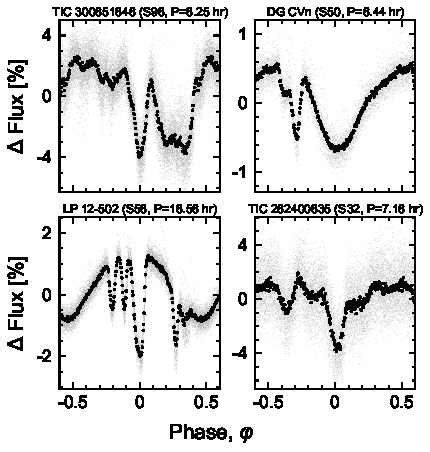
\includegraphics[width=0.48\textwidth]{lc_mosaic_mosaic4.pdf}
  \vspace{-0.4cm}
  \caption{{\bf The targets.}  We acquired new spectra and multi-color
  photometry for four complex periodic variables: TIC~300651846,
  DG~CVn (TIC~368129164), LP~12-502 (TIC~402980664), and
  TIC~262400835.  Panels show one month of TESS data folded on each
  object's period,
  with 120-second cadence flux measurements in gray and their average
  in black.  For DG~CVn, we removed a best-fit sinusoid to the
  $P_2$=2.60\,hr secondary companion's rotation signal (3.1\,AU
  projected separation; \citealt{Beuzit2004}).  The time
  evolution of each target from 2018--2025 is shown in the
  associated \href{https://lgbouma.com/cgcd_2026}{{\bf online
  movies}}: while the periods remain fixed, the morphologies evolve
  over months to years.}
  \label{fig:lcmosaic}
\end{figure}


Complex periodic variables (CPVs) present the kind of signal that
astronomers usually consider easy: large amplitude, short period, and
repeatable.  Yet a decade after their discovery, the composition,
structure, and origin of the occulting material remain unestablished.
These issues are worth resolving.  CPVs are young M dwarfs, and the
occulting material trapped in their magnetospheres exist at a few stellar
radii: the region occupied by the closest planets, and an environment
that is otherwise hard to measure.  Stars alter planets with both light
and particles.  While the impact of stellar photons on exoplanets is widely
appreciated \citep{France2016,Owen2019}, the particle environment can
be just as influential \citep{Catling2017}, and means for studying it
are scarce \citep{Loyd2025}. A star that traps circumstellar material
where we can watch it transit is as close to a space-weather station
as nature provides.

Figure~\ref{fig:lcmosaic} shows the main objects of interest in this
article; over one hundred analogous systems have been reported by K2
and TESS
\citep{Rebull2016,Stauffer2017,Rebull2018,Zhan2019,Rebull2020,Stauffer2021,Palumbo2022,Popinchalk2023,Bouma2024}.
CPVs are identified phenomenologically from their structured, periodic
optical light curves; most are M dwarfs with rotation periods shorter
than two days, and within current sensitivity limits, none host disks
\citep{Stauffer2017,Bouma2024}.  About 3\% of stars a few million
years old show the behavior, declining to $\approx$0.3\% by
$\approx$110\,Myr \citep{Rebull2020}.  
The leading interpretation is that clumps of charged circumstellar material
corotate with the star \citep{Stauffer2017}.
The physical requirement is a 
``centrifugal magnetosphere'' \citep[e.g.][]{Petit2013}:
when the magnetospheric radius exceeds the corotation radius, the
effective potential along closed field lines acquires local minima
beyond corotation where charged material can accumulate.  The
accumulation occurs in warped
tori for tilted dipoles \citep{Townsend2005}, and more complex
surfaces for multipolar fields \citep{Krticka2022}. 

Spectroscopy offers a direct test of the corotating-material
hypothesis, and the necessary data have only recently become
available.
Early spectroscopic characterization of CPVs was single-shot
reconnaissance, and established the
class as ``weak-lined T~Tauri'' stars
\citep{Stauffer2017} that were 
chromospherically active with no evidence for accretion.
The first time-series spectroscopy of a CPV showed additional sinusoidal-in-time
H$\alpha$ emission at circumstellar velocities, tracing cool
($\lesssim$10$^4$ K) plasma clumps at opposing stellar longitudes near
2-4\,$R_\star$, consistent with a pinched torus of magnetospherically
trapped plasma \citep{Bouma2025}. 
Similar Balmer emission variability is known among rapid magnetic
rotators across a wide range of masses
\citep{Donati2000,Townsend2005b,Dunstone2006,Skelly2008}, as is a
complementary absorption phenomenology
\citep{CollierCameron1989,CollierCameron1992,Cang2020}.   Yet those
stars do not show complex photometric variability, and before this
work, TIC~141146667 was the only unambiguous CPV reported to show
both, leaving the question of universality open.
Do all CPVs harbor 
bound plasma?  Which of the observed morphological features, such as
opposing clumps, night-to-night variability, or Balmer extinction
during transits, generalize across the class?

While spectroscopy can reveal the gas, multicolor photometry provides
independent evidence for what causes the dips.
Ground-based campaigns have established that CPV dips
deepen toward the blue, with power-law slopes $\beta$$\approx$0--1.5
for $\delta \propto \lambda^{-\beta}$
\citep{Onitsuka2017,Tanimoto2020,Gunther2022,Koen2023}.  
This behavior suggests extinction by sub-micron dust.
Three issues, however, complicate this interpretation.
Dip depths have been derived with heterogeneous detrending choices,
which propagate into the inferred chromaticity.
The dilution of the observed slope by partially opaque material has
been ignored.
And the space of considered models has typically been restricted to
simple
power laws.   The one exception was the pioneering
study by \citet{Tanimoto2020}, who explored broken extinction laws for
PTFO~8-8695, albeit interpreting the CPV in that system
\citep{Bouma2020} as a planet candidate.
These limitations matter because the chromaticity is an observable
that is directly linked to the question of where the dust in
these systems comes from.  Are these M dwarfs condensing out dust within
their own magnetospheres, or trapping the detritus of planet
formation?   Neither conclusion can be drawn without first establishing
what the occulting material does to starlight.


In this work we present time-series spectroscopy and multicolor
photometry of four CPVs (Figure~\ref{fig:lcmosaic}): 18 nights of
ground-based spectroscopy and nine nights of ground-based photometry
acquired between 2020 and 2025, usually with simultaneous TESS
coverage. 
High-resolution spectroscopy at sensitivity comparable to the
TIC~141146667 observations yields a detection of sinusoidal
circumstellar Balmer emission for a second CPV, TIC~300651846, and
upper limits for LP~12-502.  Lower-resolution spectra with
simultaneous photometry show that Balmer extinction during broadband
flux dips is ubiquitous, though often with timing offsets.
For the chromaticity, we homogeneously analyze our new photometry
together with the archival literature, placing 51 dip depths across
five stars on a common scale, and we compare four extinction-law
models.  Under the assumption that a universal extinction law applies
across the population, a broken power law between the optical and
near-infrared
is preferred; absent that assumption, models allowing star-to-star or
epoch-to-epoch variability fit as well or better.

Section~\ref{sec:obs} describes the observations and reductions;
Section~\ref{sec:results} presents the interpretation of the
spectroscopy and the extinction-law fits; Section~\ref{sec:disc}
discusses the structure and possible origins of the occulting
material; Section~\ref{sec:conc} concludes.


\section{New Observations}
\label{sec:obs}

\begin{deluxetable*}{lcccccccc}
\tablewidth{0pt}
\tabletypesize{\small}
\tablecaption{Overview of Stellar Properties\label{tab:starparams}}
\tablehead{
  \colhead{Star} &
  \colhead{$P$} &
  \colhead{$T_{\rm eff}$} &
  \colhead{$R_\star$} &
  \colhead{Age} &
  \colhead{$M_\star$} &
  \colhead{$v_{\rm eq}$} &
  \colhead{$R_{\rm c}$} &
  \colhead{Multiple?} \\[-5pt]
  \colhead{} &
  \colhead{(hr)} &
  \colhead{(K)} &
  \colhead{($R_\odot$)} &
  \colhead{(Myr)} &
  \colhead{($M_\odot$)} &
  \colhead{(\kms)} &
  \colhead{($R_\star$)} &
  \colhead{}
}
\startdata
TIC\,300651846 & 8.25  & $3159^{+56}_{-84}$ & $0.61^{+0.04}_{-0.03}$ & 23 & $0.40^{+0.02}_{-0.03}$ & $89.8 \pm 5.2$  & $2.49 \pm 0.15$ & N \\
LP\,12-502     & 18.56 & $3090^{+31}_{-59}$ & $0.37^{+0.02}_{-0.01}$ & 80          & $0.22^{+0.01}_{-0.02}$ & $24.2 \pm 1.0$  & $5.78 \pm 0.27$ & N \\
DG\,CVn        & 6.44  & $3127^{+51}_{-42}$ & $0.72^{+0.02}_{-0.03}$ & 150         & $0.40^{+0.02}_{-0.06}$ & $135.8 \pm 4.7$ & $1.79 \pm 0.09$ & Y \\
TIC\,262400835 & 7.16  & $3074^{+64}_{-58}$ & $1.00^{+0.04}_{-0.05}$ & 19 & $0.30^{+0.03}_{-0.04}$ & $169.6 \pm 7.6$ & $1.26 \pm 0.07$ & Y \\
\enddata
\tablecomments{DG\,CVn is TIC\,368129164; LP\,12-502 is
  TIC\,402980664.  
	Following \citet{Bouma2024}, effective temperatures and radii are from SED
fits and masses are from PARSEC isochrones \citep{Chen2014}.
  This procedure may yield biased results for binaries unresolved in
  the underlying photometry ({\it i.e.},~for the latter two systems).
	The age for LP~12-502 comes from co-moving pre-main sequence stars in its
	vicinity \citep{Tofflemire2021};
	ages for the remaining stars are from association memberships
	\citep{Gagne2026} and have relative uncertainties $\approx$$\pm$15\%.  
  % 300651846 CPL8 Gagne26
  % DG CVn CVUL Gagne26
  % LP 12-502 comove
  % TIC 262400835 greater Taurus Kerr2021
  The equatorial velocity $v_{\rm eq}$$=$$2\pi R_\star/P$ and the
  Keplerian corotation radius $R_{\rm c}$$=$$(G M_\star
  P^2/4\pi^2)^{1/3}$ are derived quantities.  The
  multiplicity column is Yes/No:
  DG\,CVn is a resolved binary (3.1\,AU projected separation;
  \citealt{Beuzit2004}) in which one component is the CPV;
  TIC\,262400835 is likely an unresolved pair within a hierarchical
  triple (see text).}
\end{deluxetable*}





\subsection{Selection Function}
\label{sec:selfn}

We chose CPVs for spectroscopic and photometric follow-up by
considering known CPVs in the literature and selecting on the
basis of target brightness, period, morphology, accessibility for
simultaneous photometry, and binarity
\citep{Rebull2016,Stauffer2017,Rebull2018,Zhan2019,Rebull2020,Stauffer2021,Palumbo2022,Popinchalk2023,Bouma2024}.
We weighted these factors as follows.

\begin{enumerate}[label={\it \roman*)},leftmargin=12pt,topsep=0pt,itemsep=-1ex,partopsep=1ex,parsep=1ex]
	\item {\it Brightness:} Brighter stars provide more photons,
	enabling higher S/N measurements.
	%
	\item  {\it Period:} Shorter periods are better, in that they enable
	covering a larger fraction of a cycle in a single night's observations.
	Since the morphologies are unpredictable over timescales of more
	than a few weeks, maximizing the duty cycles maximizes the
	probability of observing during a sharp, ``complex'', dip.
	%
  \item {\it Morphology:} We selected CPVs that showed sharp dips with large amplitude; such
  features can be most easily distinguished from spot-induced
  variability.   The desire for sharp dips can be in tension with the
  desire for short periods, as the shortest period CPVs tend to have
  smoother features (the origin of the \citet{Stauffer2017} ``scallop''
  designation). 
  %
  \item {\it Accessibility:} We favored targets close to the TESS
  continuous viewing zones, since they offered a greater number of
  schedulable windows for simultaneous photometry and spectroscopy.
  %
  \item {\it Binarity:} We were agnostic to binarity, provided that
  there was no evidence for close ($<$0.1\,AU) binarity that
  might influence the immediate circumstellar environment of either
  star.  While the CPV binary fraction is similar to that of
  the field \citep{Bouma2024}, no CPVs in such close binaries are currently known. 
\end{enumerate}

Applying these considerations to the full census yielded five targets
for our program: LP\,12-502, DG\,CVn, TIC\,300651846, and TIC\,262400835
have new data presented in this work; 
TIC\,141146667 was discussed in \citet{Bouma2025}.
Table~\ref{tab:starparams} summarizes the stellar properties,
while
Tables~\ref{tab:obs_spec} and~\ref{tab:obs_phot} summarize our
spectroscopic and photometric observations.  Most of these
stars are best-in-class in at least one of the above dimensions:
LP\,12-502 in morphology, TIC\,300651846 in southern accessibility,
DG\,CVn in brightness (due to it being the closest CPV system known, and
also a binary), and TIC\,141146667 for its short 3.9\,hour period and
relative brightness.  

This work is the first to highlight TIC~262400835
(Gaia~DR3~3234917110482839680) as a CPV.  Although \citet{Bouma2024}
noted the source, it was omitted from that catalog because automated
methods did not recover it; it was instead found in 2020 through the
CDIPS project \citep{Bouma2019}.  Its short period and complex
morphology motivated two-minute and 20-second cadence observations in
DDT028, during which we also acquired MuSCAT1 and MuSCAT2 photometry.
Since then, \citet{Kerr2021} reported the system as being
part of the $\approx$19\,Myr old ``Greater Taurus Subgroup 3A'', a
designation which the latest MocaDB BANYAN-$\Sigma$ models support
\citep{Gagne2026}.  The system is likely a triple.
There is a resolved companion, Gaia DR3 3234920065420339712
(ATO~J078.4822+02.6114, TIC 262400836), 10$\farcs$6 due West
(projected separation $\sim$1{,}800\,AU), with consistent parallax and
proper motion.  The companion is 0.3\,magnitudes bluer in BP-RP, and
thus is likely the primary despite having a near-identical $G$-band
magnitude.  Our seeing-limited photometry shows that TIC~262400835 is
the host of the complex variability; it is likely an unresolved pair
on the basis of its Gaia DR3 RUWE (1.5) and photometric excess.  The
triple interpretation is also consistent with the TESS data, which
within a single 20$''$ pixel show three distinct periods: the
large-amplitude complex signal at $P_1$=7.16\,hr; a $P_2$=4.31\,day
slow sinusoidal signal; and a faster $P_3$=12.70\,hr
sinusoidal signal.  As described below, the MuSCAT1 and MuSCAT2 data
enable associating the 7.16\,hr signal to TIC~262400835
(Gaia~DR3~3234917110482839680), which is sufficient for the aims of
this article.  \citet{Heinze2018} report the neighbor, TIC~262400836,
as a $P$=4.3\,day close binary; we concur with the period but see no
evidence for eclipses at that period in the TESS light curves.


\begin{deluxetable*}{llllcccc}
\tablewidth{0pt}
\tabletypesize{\small}
\tablecaption{Spectroscopic Observations\label{tab:obs_spec}}
\tablehead{
  \colhead{Star} &
  \colhead{Spectrograph} &
  \colhead{Photometer} &
  \colhead{Night} &
  \colhead{$\Delta R$ for} &
  \colhead{Circ.\ Gas} &
  \colhead{H$\alpha$ Dips} &
  \colhead{Flare-Induced} \\[-5pt]
  \colhead{} &
  \colhead{} &
  \colhead{} &
  \colhead{(UT)} &
  \colhead{Circ.\ Gas?} &
  \colhead{in Emission?} &
  \colhead{with Flux Dips?} &
  \colhead{Spec.\ Var.?}
}
\startdata
LP\,12-502                            & DBSP  & Tierras & 2023 Nov 11 & $\times$     & $\times$            & $\checkmark$ & $\checkmark$ \\
LP\,12-502                            & DBSP  & Tierras & 2023 Nov 12 & $\times$     & $\times$            & $\checkmark$ & $\checkmark$ \\
LP\,12-502                            & DBSP  & $\times$ & 2023 Dec 07 & $\times$     & $\times$            & -- & -- \\
LP\,12-502                            & DBSP  & TESS    & 2024 Nov 04 & $\times$     & $\times$            & $\checkmark$ & $\checkmark$ \\
LP\,12-502                            & DBSP  & TESS    & 2024 Nov 05 & $\times$     & $\times$            & $\times$ & $\checkmark$ \\
LP\,12-502                            & DBSP  & TESS    & 2024 Nov 06 & $\times$     & $\times$            & $\times$ & $\checkmark$ \\
LP\,12-502                            & DBSP  & TESS    & 2024 Nov 07 & $\times$     & $\times$            & $\checkmark$ & $\checkmark$ \\
LP\,12-502                            & DBSP  & TESS    & 2024 Nov 08 & $\times$     & $\times$            & $\times$ & $\checkmark$ \\
LP\,12-502                            & HIRES & $\times$ & 2023 Nov 23 & $\checkmark$ & $\times$            & -- & -- \\
LP\,12-502                            & HIRES & TESS    & 2024 Dec 03 & $\checkmark$ & $\times$            & $\checkmark$ & $\checkmark$ \\
LP\,12-502                            & HIRES & TESS    & 2024 Dec 10 & $\checkmark$ & $\times$            & $\times$ & $\checkmark$ \\
DG\,CVn                               & DBSP  & Tierras & 2024 Apr 28 & ?            & $\times$            & $\checkmark$ & $\times$     \\
TIC\,300651846                        & MIKE  & TESS    & 2025 Jan 02 & $\checkmark$ & $\checkmark$        & $\checkmark$ & $\times$     \\
TIC\,300651846                        & MagE  & TESS    & 2025 Jan 18 & $\checkmark$ & $\checkmark$        & $\checkmark$ & ?            \\
TIC\,300651846                        & MagE  & TESS    & 2025 Jan 19 & $\checkmark$ & $\checkmark$        & $\checkmark$ & $\times$     \\
TIC\,300651846                        & MagE  & TESS    & 2025 Jan 20 & $\checkmark$ & $\times$            & $\checkmark$ & $\times$     \\
TIC\,300651846                        & MagE  & TESS    & 2025 Jan 21 & $\checkmark$ & $\times$            & $\checkmark$ & $\times$     \\
TIC\,141146667$^{\dagger}$            & HIRES & TESS    & 2024 Feb 17 & $\checkmark$ & $\checkmark$        & $\checkmark$ & ?     \\
\enddata
\tablecomments{ The latter four columns indicate (i) whether the
  spectrograph had sufficient resolution relative to the stellar
  equatorial velocity to resolve bound circumstellar gas in emission, (ii)
  whether such gas was seen, (iii) whether the H$\alpha$
  equivalent width time series showed dips synchronous with broadband
  flux dips, and (iv) whether the spectra and photometry showed synchronous evidence for
  flare-induced variability.  $^{\dagger}$Data for TIC~141146667 were
  described in \citet{Bouma2025}.}
\end{deluxetable*}



\subsection{Magellan/MagE}
\label{sec:mage}

We observed TIC~300651846 ($V$=14.1) over four consecutive nights
spanning 18~January to 21~January~2025 using the Magellan Echellette
(MagE; \citealt{Marshall2008}) spectrograph on the Baade 6.5\,m
Magellan telescope.  We used the 1$''$$\times$10$''$ slit
($R$$\approx$4{,}100, $\delta v$$\approx$73\,\kms), with a 12 minute
cadence, and aligned the slit along the parallactic angle while taking
thorium-argon arcs for wavelength calibration once per hour.  The
seeing averaged 0$\farcs$8 over all four nights, rarely exceeding
1$''$.  We extracted 1-D spectra from the resulting 161 science-ready
echellograms using the CarPy data reduction package
\citep{Kelson2000,Kelson2003}, with S/N$\approx$160 per resolution
element in the continuum near H$\alpha$.  We timed these observations
to be simultaneous with TESS Sector 88.  Adopting the stellar radius
and period from \citet{Bouma2024}, TIC~300651846 has $v_{\rm
eq}$=\ticthreeveq\,\kms, implying near-critical sampling of the line
core.  Figure~\ref{fig:mage} shows the resulting time-dynamic spectra
in the vicinity of $H\alpha$, where the bottom row subtracts the
time-averaged spectrum from each night to highlight
variability---whether in the line core, or in the circumstellar
environment.  


% S/N per pixel ~87, counts 7500.
% TESS s88 overlap: 3694.5 to 3697.8

\begin{figure*}[!tp]
  \centering
  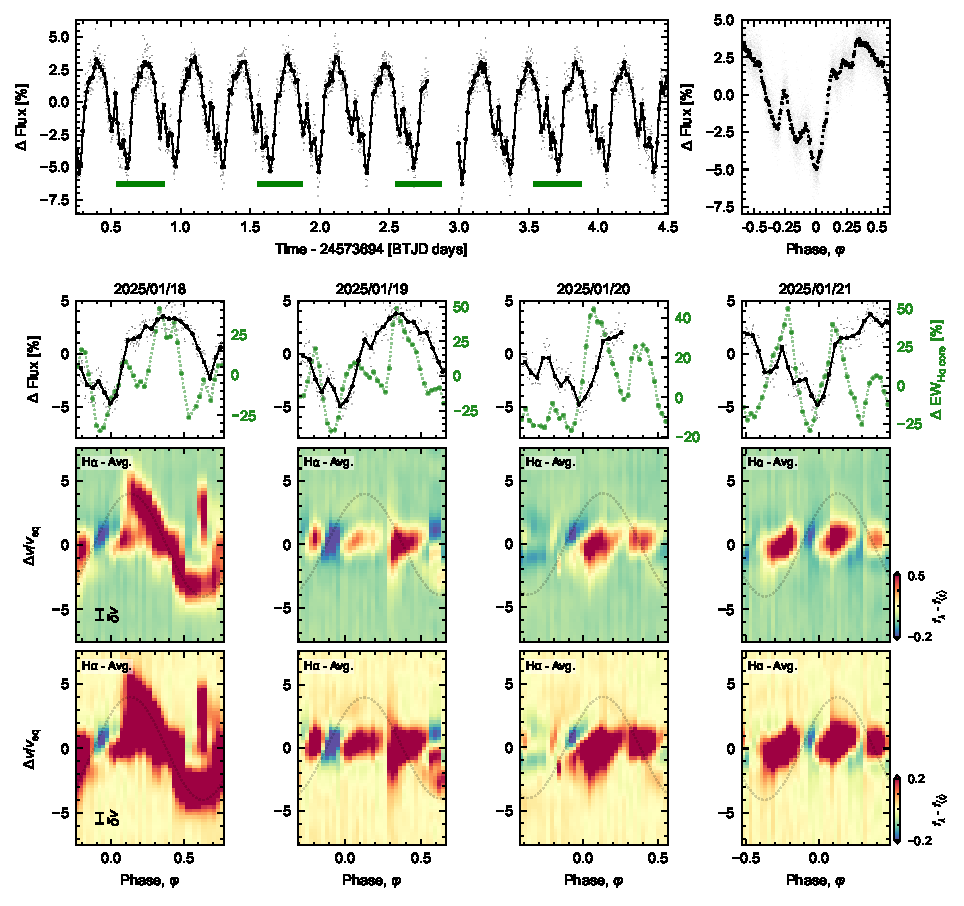
\includegraphics[width=0.99\textwidth]{mage_mosaic_simult_tworow_fournightavg.pdf}
  \vspace{-0.2cm}
  \caption{{\bf Large changes in circumstellar Balmer emission
  without any accompanying change in broadband flux morphology.} Data
  are from four successive nights on Magellan/MagE for TIC~300651846
  ($P=8.25$\,hr).  The top-left panel shows overlapping TESS data
  (raw data in gray and 20~minute time bins in black); each panel in
  the next row shows strictly simultaneous flux measurements, with the
  median-normalized H$\alpha$ line flux at $|v/v_{\rm eq}|<1$ in
  green.  
  The lower two rows show time-series H$\alpha$ profiles at two
  different color stretches, with the time-averaged mean profile 
  subtracted.  The top-right panel shows the average TESS
  light curve from 14~January~2025 to 11~February~2025.  Large
  amplitude sinusoidal-in-time Balmer emission is apparent on
  18~January 2025.  Such emission is weakly present from
  $\phi$=0.3-0.6 on 19~January and 20~January, and not detectable on
  21~January.  Despite the spectroscopic changes, the complex
  morphology in the TESS light curves remained stable.  The errorbar
  in the lower left indicates the velocity resolution.  The faint
  model is a sinusoid with $K$=4\,$v_{\rm eq}$ and $\phi_0$=-0.12.
  }
  \label{fig:mage}
\end{figure*}


\subsection{Magellan/MIKE}
\label{sec:mike}

We additionally observed TIC~300651846 on the night of 2~January~2025
using the Magellan Inamori Kyocera Echelle (MIKE;
\citealt{Bernstein2003}) spectrograph on the Clay 6.5\,m Magellan
telescope.  We used the 0.7$''$$\times$5$''$ slit, delivering
$R$$\approx$35{,}000 ($\delta v$$\approx$9\,\kms) in the red arm and
$R$$\approx$28{,}000 ($\delta v$$\approx$11\,\kms) in the blue, and
opted to read out unbinned in the spectral direction, and 2$\times$
binned in the spatial direction.  We bracketed every science
observation with a thorium-argon arc, since the main expected
advantage of this observation configuration relative to MagE was the
velocity resolution, which oversamples the line core.  The seeing over
the night averaged 0$\farcs$9.  We extracted 1-D spectra from the
resulting 23 science-ready echellograms using CarPy
\citep{Kelson2000,Kelson2003}, yielding S/N$\approx$54 per resolution
element in the H$\alpha$ continuum.  These observations were executed
simultaneously with TESS Sector 87.
Figure~\ref{fig:mike} shows the resulting time-dynamic spectra.

% 600 cts per px in red arm near Halpha continuum, 
% 5 pixels per resolution elemnt
% first observation DATE-OBS= '2025-01-03T00:46:19'        / (start)

\begin{figure}[!t]
  \centering
  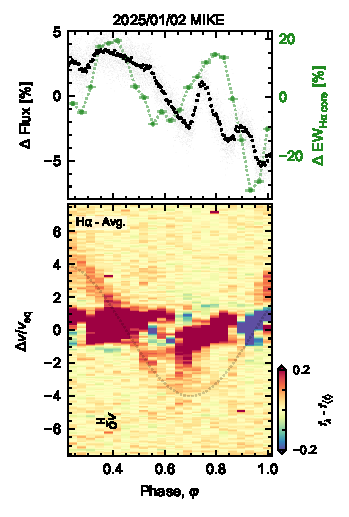
\includegraphics[width=0.45\textwidth]{mike_mosaic.pdf}
  \vspace{-0.2cm}
  \caption{{\bf Circumstellar emission for TIC~300651846 on 2~January
  mirrored 19 and 20~January. }
  The Magellan/MIKE data in this plot have eight times higher
  resolution than the MagE data in Figure~\ref{fig:mage}; we bin 
  by a factor of two in velocity for clarity, and again phase to
  $P=8.25$\,hr.
  Sinusoidal-in-time H$\alpha$ emits at $\approx$10\% of the
  continuum.
  Absorption in the line core from $\phi$=0.9-1.0 occurs during the
  transit of the corresponding clump of plasma.
  The ephemeris is the same as in Figure~\ref{fig:mage}; the
  average H$\alpha$ line profile (not shown) is similarly in emission with
  EW$=$$6.0 \pm 0.3$\,\AA.
  The faint model is a sinusoid with $K$=4\,$v_{\rm eq}$ and
  $\phi_0$=-0.05, slightly offset from Figure~\ref{fig:mage}.
  }
  \label{fig:mike}
\end{figure}


\subsection{Hale/DBSP}
\label{sec:dbsp}

We used the Double Spectrograph (DBSP; \citealt{Oke1982}) on the
Palomar 200-inch telescope (Hale/P200) to observe LP~12-502 over seven
nights: 11~November to 12~November 2023, 7~December 2023, and
4~November to 8~November 2024.  We additionally observed DG~CVn
($V$=12.0), a known unresolved binary \citep{Osten2016} in which one
component is a CPV, over the night of 28~April~2024.  We used the
1$\farcs$5 slit, with the 1200 line/mm grating, blazed at 5000\,\AA\
on the blue arm, and 1200 line/mm, blazed at 7100\,\AA\ on the red
arm.  This delivered $R$$\approx$2{,}200 at H$\alpha$, corresponding
to $\delta$$v$$\approx$140\,\kms.  For LP~12-502, $v_{\rm
eq}$=\lptwelveveq\,\kms, yielding an experiment focused on equivalent
width measurement, rather than velocity resolution.  For DG~CVn
($v_{\rm eq}$=\dgcvnveq\,\kms) the velocity sampling near the line
core was near-critical.  For LP~12-502, we used 10 minute exposures,
yielding 442 spectra with 73.7 total hours of open-shutter time,
typically with S/N$\approx$200 per resolution element.  For DG~CVn, we
used six minute exposures, yielding 49 spectra over a 4.3 hour baseline.
We performed the extraction using \texttt{DBSP\_DRP}
\citep{dbsp_drp:joss}, which is an extension of the \texttt{PypeIt}
suite \citep{pypeit:joss_pub}.  We then measured the equivalent widths
of the highest S/N Balmer lines---H$\alpha$ (n=3$\rightarrow$2),
H$\beta$ (n=4$\rightarrow$2), and H$\gamma$ (n=5$\rightarrow$2)---by
numerically integrating the resulting continuum-normalized spectrum
using a one-component Gaussian with free amplitude, width, and mean.  We
estimated the uncertainties on each line width through a Monte Carlo
procedure that bootstrapped against the local scatter in the continuum. 

The two LP~12-502 nights in November 2023 were conducted
simultaneously with the Tierras photometer at FLWO
\citep{Garcia-Mejia2020}, detailed in Section~\ref{sec:tierras} below.
The remaining observations, save for 7~December 2023, were conducted
simultaneously with TESS.  Figure~\ref{fig:dbsp} summarizes the
results from the most informative nights: 11~November to 12~November
2023, 4~November and 7~November 2024 for LP~12-502, and 28~April 2024
for DG~CVn.  Figure~\ref{fig:dbsp_detail} provides further detail on
the H$\alpha$, H$\beta$, and H$\gamma$ equivalent widths and line
profiles for the November 2023 nights.  Data from the remaining nights
of 5~November and 6~November 2024 for LP~12-502 are presented in
Appendix~\ref{app:ootspec}---these observations covered
orbital phases with no ``complex'' flux dips; only a single broadband
flare on 5~November yielded a corresponding spike in the Balmer lines
similar to those visible in Figure~\ref{fig:dbsp}.  The night of
7~December 2023 yielded viable DBSP data, but a TESS perigee contact
extended into the DBSP observation, yielding insufficient overlapping
photometry for further analysis.

% Nov05,Nov06 2024 - where just at an orbital phase that showed no flux dips

% Dec07 2023: poor TESS coverage due to orbit contact.  SAP_FLUX S73
% available starting BJDTDB 2460285.801.
% This only covers the latter third of the DBSP data, and the majority
% of variability in DBSP, likely including a large flare, happens
% before TESS data are available.

% DBSP LP12-502: extracted spectra showing 10-25k counts per pixel near
% Halpha continuum, depending on seeing and airmass

\begin{figure*}[p]
  \centering
  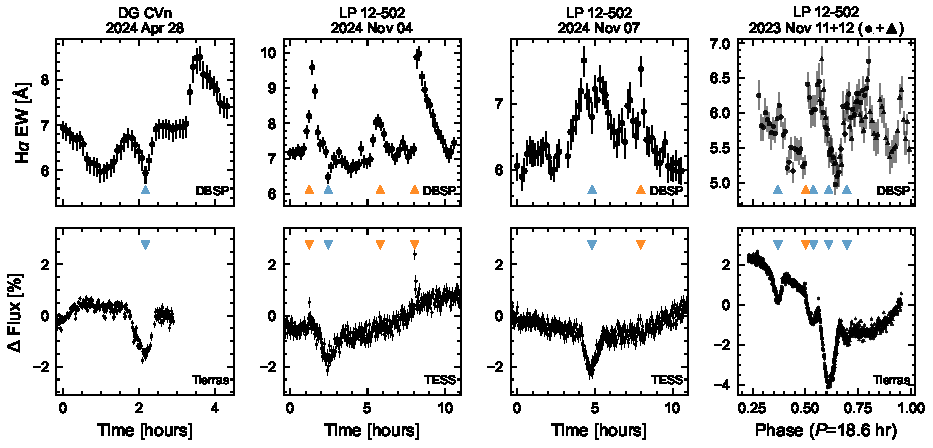
\includegraphics[width=0.98\textwidth]{DBSP_HAlpha_mosaic.pdf}
  \vspace{-0.2cm}
  \caption{{\bf CPVs show Balmer line extinction during broadband
  transits---however, Balmer variability is dominated by flares.}
  Panels show Hale/DBSP ($R$$\approx$2{,}200) H$\alpha$ equivalent
  widths (EWs) vs.~simultaneous Tierras and TESS photometry.
  Minute-timescale optical flares (orange arrows) are associated with hour-timescale
  Balmer EW flares.  The $\sim$hour timescale
  optical dips that define the CPV class (blue arrows) tend to be contemporaneous
  with Balmer EW dips, consistent with transiting clumps of dusty plasma
  (see discussion in Section~\ref{sec:dustyplasma}).
  The rightmost column is shown as a function of phase since the data
  were acquired two orbital cycles apart.
  }
  \label{fig:dbsp}
\end{figure*}

\begin{figure*}[p]
  \centering
  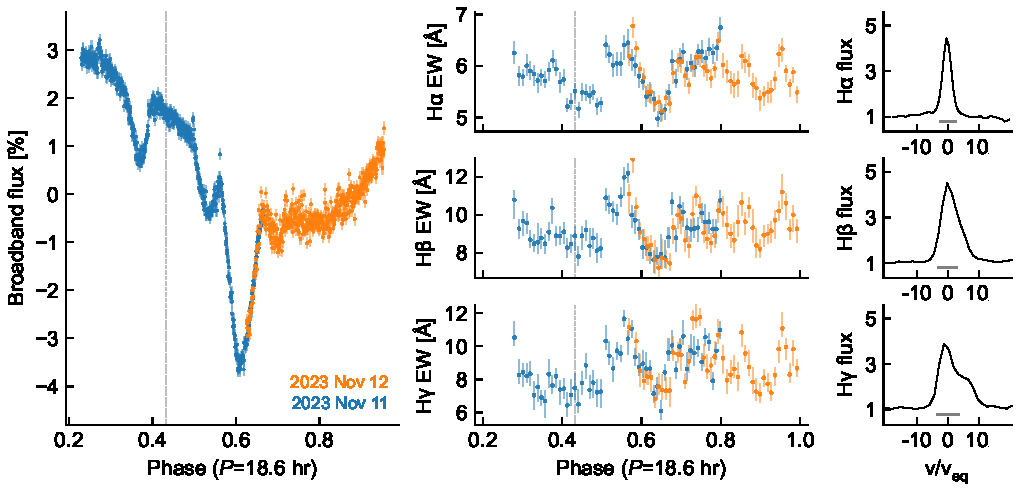
\includegraphics[width=0.98\textwidth]{dbsp_20231111_20231112_frame.pdf}
  \vspace{-0.2cm}
  \caption{{\bf Detail of Figure~\ref{fig:dbsp}, showing H$\alpha$,
  H$\beta$, and H$\gamma$ equivalent widths and line profiles for
  LP~12-502 on 11 and 12 November, 2023.} The
  \href{https://lgbouma.com/movies/LP_12-502_dbsp_Nov2023.mp4}{{\bf
  online movie}} shows the line profiles for each exposure,
  switching from Nov~11 to Nov~12 near
  $\phi$$\approx$0.8.  The target, LP~12-502, has 
  $v_{\rm eq}$=24.2\,km/s; gray horizontal lines denote a single
  velocity resolution element ($\delta$$v$$\approx$$c$/R).  The Balmer
  line equivalent widths vary at the 5-50\% level, coincident in time
  with 1-2\% variability in the broadband Tierras filter.  There is
  strong evidence for line shape differences between H$\alpha$,
  H$\beta$, and H$\gamma$, and weak evidence for time variability in
  the velocity-resolved emission profile of H$\gamma$.  The jump at
  $\phi$$\approx$0.50 was likely flare-induced, based on similar
  timing coincidences in Figure~\ref{fig:dbsp}.}
  \label{fig:dbsp_detail}
\end{figure*}


\subsection{Keck/HIRES}
\label{sec:hires}

We observed LP~12-502 ($V$=13.9) over 23~November~2023,
3~December~2024, and 10~December~2024 using the High Resolution
Echelle Spectrometer (HIRES; \citealt{vogt_hires_1994}) on the 10\,m
Keck I telescope.  We used the C2 decker
(0$\farcs$86$\times$14$\farcs$0) in the red configuration, yielding a
resolution $R$$\approx$45{,}000 ($\delta v$$\approx$6.7\,\kms).  The
seeing averaged 1$\farcs$2, 1$\farcs$6, and 2$\farcs$1 in each
respective night, with strong winds in the latter two nights.
% S/N 40-70 per pixel; 3 pixels per resolution element along dispersion.
With 15-20 minute cadence, this configuration delivered an S/N of
70-120 per resolution element in the H$\alpha$ order's continuum, and
a total of 20.1\,hours of open-shutter time.  The
star's radius and period from \citet{Bouma2024} imply an equatorial
velocity (2$\pi$$R_\star$/$P$) of $v_{\rm eq}$=\lptwelveveq\,\kms, so
the instrument provided a few resolution elements across the line
core.  We reduced the echellogram using the standard techniques of the
California Planet Survey \citep{Howard2010}.  

We acquired simultaneous photometry for the December~2024 nights by
observing simultaneously with TESS.  We attempted to acquire
near-simultaneous Tierras observations for the November~2023 night but
had poor weather in Arizona.
We detail the results in Appendix~\ref{app:ootspec}.
In short, while the HIRES spectra and photometry of LP~12-502
presented abundant evidence for flare-induced variability, we observed
only a $\approx$one hour partial transit of a single ``complex'' dip,
which was coincident with excess absorption in Balmer line cores.

% NOTES:
% 23Nov2023: 05:41 - 13:17 UT j531.logsheet1, ~1.2", ~19k ct/exp, texp 1200, continuum near Ha shows 5k ct per px.
% 03Dec2024: 04:54 - 10:07 UT j546.logsheet2, ~1.6" windy, ~2.5k ct/exp, texp 900
% 10Dec2024: 04:28 - 11:48 UT j547.logsheet1, ~2.1" windy, ~2.5k ct/exp, texp 1200, continuum near Ha 2.8k ct per px




\subsection{Hale/TSPEC}
\label{sec:tspec}

{\bf Facundo:  To report, or not to report?  And what to say?  It's a
few usable spectra, with little ability to assess time variability.
However, they could still be useful for the limit on spot-covering
fraction.  I could go either way.}

% TODO: instrument config (cross-dispersed NIR, 0.94--2.46\,\micron,
% R~2500), observing conditions, exposure times, nodding/dithering
% pattern, and reduction (Spextool or custom).

\subsection{Magellan/FourStar}
\label{sec:fourstar}

We observed TIC~300651846 ($K$\,=\,10.8) on 11~February~2025 (UT) using
FourStar \citep{Persson2013}, a near-infrared wide-field imager on
the Baade 6.5\,m Magellan telescope.  We used the NB2.09 narrowband
filter ($\lambda$\,=\,2.082--2.118\,$\mu$m), in the Double read mode,
taking 20.38\,s exposures.  The broader
$K$-band filter would have saturated the detector given the target's
brightness.  Young M dwarfs present no prominent emission or
absorption lines within the NB2.09 bandpass: the H$_2$ 1--0\,S(1)
transition at 21{,}218\,\AA\ falls off-band.  Variability detected in
this filter can therefore be interpreted as continuum variability.

Humidity kept us closed over the first quarter of the night.  After
opening, we observed continuously for 5.3\,hr beginning at BJD$_{\rm
TDB}$\,=\,2460717.650, with seeing averaging 0$\farcs$9.  We reduced
the images to light curves using {\tt AstroImageJ}
\citep[][]{Collins2017} and converted timestamps from JD$_{\rm UTC}$
to BJD$_{\rm TDB}$ using the \citet{Eastman2010} barycentric
correction code.  Figure~\ref{fig:fourstar} shows the resulting light
curve phased to $t_0$\,=\,BJD$_{\rm TDB}$\,2460693.244 and
$P$\,=\,0.34392\,d (8.25\,hr), with the simultaneous TESS observation
from Sector~88.

\begin{figure}[htp!]
  \centering
  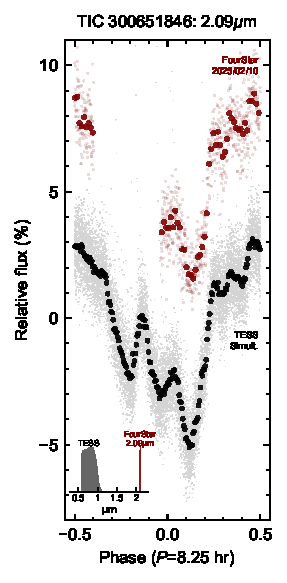
\includegraphics[width=0.48\textwidth]{fourstar_vs_tess_phase.pdf}
  \vspace{-0.4cm}
  \caption{{\bf Magellan/FourStar 2.09\,$\mu$m 
  vs.~simultaneous TESS (0.6-1\,$\mu$m) observations.}  The target,
  TIC~300651846, has a period of 8.25 hours and was observable for
  two-thirds of a rotation cycle with FourStar on 11~February~2025.
  Simultaneous TESS data from Sector 88 are plotted underneath.  The
  two bands (filter profiles in lower left) show dip depths in a ratio
  of \fourstarobsratio$\pm$\fourstarobsratiounc\ (NB2.09/TESS).}
  \label{fig:fourstar}
\end{figure}

\begin{figure}[htp!]
  \centering
  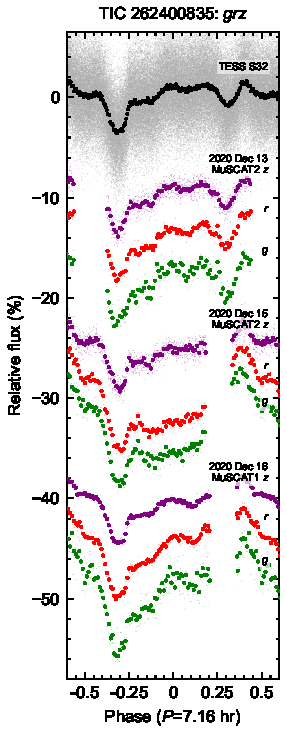
\includegraphics[width=0.45\textwidth]{TIC262400835_multicolor_phase_stacked.pdf}
  \vspace{-0.3cm}
  \caption{{\bf MuSCAT1 and MuSCAT2 $g'r'z_{\rm s}$ vs.~simultaneous TESS observations.}  The
  target, TIC~262400835, has a period of 7.16 hours.  The plotted TESS
  data, acquired at 20 second cadence, span 19 November 2020 to 17
  December 2020.}
  \label{fig:muscat}
\end{figure}


\subsection{MuSCAT1 and MuSCAT2}
\label{sec:muscat}

We observed TIC~262400835 on 13 and 15~December~2020 UT using the
MuSCAT2 multi-band imager \citep{Narita2019} mounted on the 1.5\,m
Telescopio Carlos S\'{a}nchez (TCS) at Teide Observatory, Spain.
MuSCAT2 is equipped with four CCDs capable of obtaining simultaneous
imaging in the $g'$, $r'$, $i'$, and $z_{\rm s}$ bands with negligible
readout overhead. Each CCD consists of $1024 \times 1024$ pixels,
providing a field of view of $7.4 \times 7.4$\,\arcmin$^{2}$.

We conducted the MuSCAT2 observations with the telescope in nominal
focus. On both nights, we set the exposure times to 60\,s for the
$g'$, $r'$, and $i'$ bands, and 15\,s for the $z_s$ band.  We
processed the raw data using the MuSCAT2 pipeline
\citep{Parviainen2019}, which performs standard dark and flat-field
calibrations followed by aperture photometry.   We also used this
pipeline to model instrumental and environmental systematics,
specifically accounting for variations induced by airmass changes and
pixel-positional shifts due to telescope guiding.  We adopted
identical reference stars across both MuSCAT2 nights, and adopted an
aperture with $r$=16\,px ($7\farcs0$) to ensure negligible
contamination from TIC~262400836.  This aperture choice localized
the 7.16\,hr ``dip'' signal to TIC~262400835.

We also observed TIC~262400835 on the night of 16~December~2020 UT using
MuSCAT1 \citep{Narita2015}, a multi-band imager on the 1.88\,m
telescope at Okayama Astrophysical Observatory (OAO), Japan.  MuSCAT1
is equipped with three CCDs, enabling simultaneous imaging in the
$g'$, $r'$, and $z_s$ bands with negligible readout overhead. Each CCD
provides a field of view of $6.1 \times 6.1$\,arcmin$^2$ over $1024
\times 1024$ pixels.

We used exposure times of 60 seconds in the $g'$, $r'$, and $z_{\rm s}$
bands.  We dark-subtracted and flat-fielded the raw images, and
performed aperture photometry following \citet{Fukui2011}, adopting an
aperture radius of 8, 10, and 14\,px ($2\farcs9$, $3\farcs6$, and
$5\farcs1$) to exclude the flux of the companion $\sim$10\arcsec\
to the West. These observations were conducted simultaneously with
TESS Sector 32, and the resulting light curves are shown in
Figure~\ref{fig:muscat} alongside the MuSCAT2 data.



\subsection{KeplerCam}
\label{sec:keplercam}

\begin{figure}[!t]
  \centering
  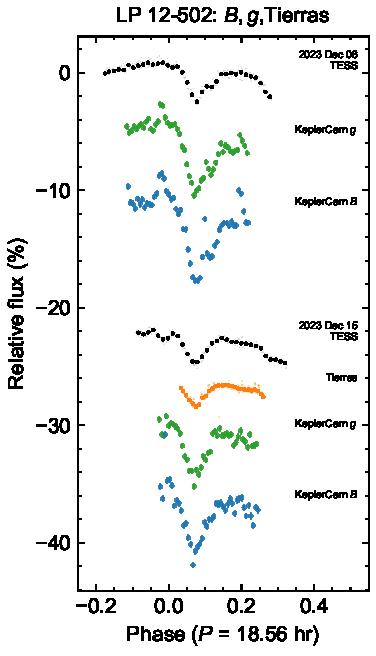
\includegraphics[width=0.48\textwidth]{LP12502_multicolor_phase_stacked_Dec08Dec15.pdf}
  \vspace{-0.4cm}
  \caption{{\bf KeplerCam $gB$ and Tierras vs.~simultaneous TESS
  observations.}  The target, LP~12-502, has a period of 18.56 hours.
  The plotted TESS data are excerpts of 120 second cadence data from
  Sector~73.}
  \label{fig:keplercamtierras}
\end{figure}

We observed LP~12-502 on 8 and 15~December 2023 UT using the KeplerCam
CCD on the 1.2\,m telescope at the Fred Lawrence Whipple Observatory
(FLWO) at Mount Hopkins, Arizona.   We took observations in
alternating $g'$ and $B$ filters with 60 sec exposure in $g'$ and 300
sec in $B$. KeplerCam is a 4096$\times$4096 Fairchild CCD which has a
field-of-view of $23\farcm1\times23\farcm1$ and an image scale of
0.672$"/$pix when binned by 2.   We reduce the data using standard IDL
routines, and performed aperture photometry using AstroImageJ
\citep{Collins2017}.
The resulting measurements are in Figure~\ref{fig:keplercamtierras}.

%  While we additionally observed on the night of 16 December 2023, there were high
%  winds and very poor seeing.   The KeplerCam $B$ and $g$ light curves
%  weakly suggest the presence of a flux dip; subsequent analysis of the
%  simultaneous TESS light curve show a $\approx$1\% deep dip lasting an
%  hour.  Due to the poor quality of these data relative to the nights of
%  8~December and 15~December, we exclude them from further analysis.

\begin{deluxetable*}{llllcc}
\tablewidth{0pt}
\tabletypesize{\small}
\tablecaption{Multicolor Photometric Observations\label{tab:obs_phot}}
\tablehead{
  \colhead{Star} &
  \colhead{Instrument} &
  \colhead{Night} &
  \colhead{Bandpasses} &
  \colhead{Dips} &
  \colhead{Chromatic?} \\[-5pt]
  \colhead{} &
  \colhead{} &
  \colhead{(UT)} &
  \colhead{} &
  \colhead{Seen?} &
  \colhead{}
}
\startdata
TIC\,262400835 & MuSCAT2             & 2020 Dec 13 & $g$, $r$, $i$, $z$, TESS      & $\checkmark$ & ?            \\
TIC\,262400835 & MuSCAT2             & 2020 Dec 15 & $g$, $r$, $i$, $z$, TESS      & $\checkmark$ & $\checkmark$ \\
TIC\,262400835 & MuSCAT1             & 2020 Dec 16 & $g$, $r$, $z$, TESS           & $\checkmark$ & $\checkmark$ \\
LP\,12-502     & KeplerCam           & 2023 Dec 08 & $B$, $g$                      & $\checkmark$ & $\checkmark$ \\
LP\,12-502     & KeplerCam + Tierras & 2023 Dec 15 & $B$, $g$, Tierras             & $\checkmark$ & $\checkmark$ \\
LP\,12-502     & KeplerCam           & 2023 Dec 16 & $B$, $g$                      & $\checkmark$ & ? \\
TIC\,300651846 & FourStar + TESS     & 2025 Feb 11 & NB2.09, TESS                  & $\checkmark$ & ? \\
\enddata
\tablecomments{``Dips Seen?'' indicates whether sharp flux dips were
  observed; ``Chromatic?'' indicates whether the dip depths differed
  significantly between bandpasses.  The FourStar entry is the
  central near-infrared constraint of this work.}
\end{deluxetable*}




\subsection{Tierras}
\label{sec:tierras}

We observed LP\,12-502 and DG\,CVn with the Tierras Observatory, a
refurbished 1.3\,m ultra-precise fully-automated photometer located at
the F.~L.\ Whipple Observatory atop Mount Hopkins, Arizona
\citep{Garcia-Mejia2020}. The facility carries out all observations
through a single custom narrow bandpass filter ($\lambda_C =
863.5$~nm, FWHM $= 40$~nm) that minimizes precipitable water vapor
(PWV) errors known to limit photometric precision from the ground
\citep[e.g.,][]{Stubbs2007,Blake2008,Berta2012}. Tierras is also
equipped with a deep-depletion $4\mathrm{K} \times 4\mathrm{K}$ e2v
CCD ($15~\mu$m pixels) with a plate scale of $0\farcs43$~pixel$^{-1}$
operated in frame-transfer (shutter-less) mode, yielding a field of
view (FOV) of $15' \times 29'$.

We observed LP\,12-502 during the UT nights of 11~November,
12~November, and 15~December 2023, as well as DG\,CVn on the UT night
of 28 April 2024.  The telescope was in focus throughout.  We exposed
for 45~s on LP\,12-502, collecting 556, 421, and 296 frames over 8.1,
6.1, and 4.2~hr, respectively, and for 30~s on DG\,CVn, collecting 731
frames over 7.9~hr. Our LP\,12-502 observations sampled airmasses
between 1.52 and 1.74, a consequence of the target's high declination
($+80\fdg5$), which renders it circumpolar from Mount Hopkins, while
our DG\,CVn observations sampled airmasses between 1.00 and 1.80.
Skies were clear on all four nights, with relative humidities between
10\% and 52\%. The median image FWHM was $0\farcs9$, $1\farcs7$,
$1\farcs3$, and $1\farcs1$, listed chronologically.

We produced light curves from the Tierras images using the facility's
pipeline, which we briefly summarize here. The pipeline first
bias-corrects the images by subtracting bias levels derived from the
overscan region of each detector half, each of which is read through a
separate amplifier, and it subsequently stitches the two halves
together. We did not flat-field the data given that, when these
observations were gathered, light entering the Tierras optical path
off-axis produced an additive glow that a flat field would not have
corrected. This effect has since been suppressed with additional
internal baffling.  We then computed an astrometric solution for each
frame, and extracted photometry for stars brighter than $G_\mathrm{RP}
= 17$~mag.  We measured fluxes through a family of circular apertures
spanning 5 to 20~pixels in radius, and estimated the local sky in each
case from an annulus running from 35 to 55~pixels, taking the
$2\sigma$-clipped median of the pixels it encloses.  Our per-frame
error budget combined photon noise from the star and from the sky with
dark current, read noise, and scintillation \citep{Stefansson2017}.
We discarded frames in which the target flux encroached on the
detector's non-linear regime, which is why only 609 of the 731 DG\,CVn
frames were kept for the subsequent analysis.  We retained all 1273
LP\,12-502 frames.

Finally, we normalized our target fluxes by a weighted sum over the
ensemble of comparison stars, with the weights set by the iterative
scheme detailed in \citet{Tamburo2022}.  In this scheme, stars that
contribute noise are progressively downweighted until the weights stop
changing.  We then freeze the converged weights and reuse them for
every night of a given target. Holding the ensemble fixed in this way
guarantees that a brightness change measured for a variable target
between two nights cannot be an artifact of shifts in the comparison
set. For each target we kept the aperture that minimized the measured
scatter: 17~pixels ($7\farcs3$) for LP\,12-502, with an ensemble of
403 comparison stars, and 10~pixels ($4\farcs3$) for the brighter
DG\,CVn, with 86 comparison stars. Individual exposures for the two
targets reach a photometric precision of 1.1 to 1.7~ppt.


\subsection{Dip Depth Measurement}
\label{sec:dipfit}

We measured the depth, mid-time, and duration of each dimming event
in the ground-based photometry by treating
every observed dip independently.  We fitted the light curves using a
two-stage least squares routine.  We first manually provided a guess
for which points were ``in-dip'', which neighboring points provided
the ``out-of-dip'' baseline, and which points to exclude due to
flaring.  We constrained this initial guess to be identical across
bandpasses.  We then fit a smooth rotational baseline, $b(t)$, to only
the out-of-dip points, and subsequently fit the residual, $f(t) -
b(t)$, with a dip model.  We explored various models for the
rotational baseline (low-order polynomial; low-order Fourier series)
and the dip model (hyperbolic secant per \citealt{Yu2015}; trapezoidal
dip), always requiring the dip epoch and total duration to be
identical over bandpasses, but letting the depth and shape parameters
vary.  We assessed the goodness of fit for each model using the
reduced $\chi^2$, as initially evaluated by setting the flux
uncertainties to the point-to-point out-of-dip RMS (the 84$^{\rm
th}$-16$^{\rm th}$ percentile spread of the first differences $\Delta
F_j = F_j - F_{j+1}$), and subsequently renormalized to force the
best-fitting model to have $\chi^2_{\rm red} \equiv 1$.  We then
compared the model evidence using the Bayesian Information Criterion
(BIC).  We found across all the photometric datasets that at most
second-order baseline models minimized the BIC, and that the
trapezoidal dip model (parametrized by depth, duration, mid-time, and
fractional ingress/egress duration) offered better $\chi^2_{\rm red}$
and $\Delta {\rm BIC}$ than the hyperbolic secant (parametrized by
depth, width, and mid-time).  Table~\ref{tab:dipdepths} lists the
resulting depth measurements, based on the trapezoidal model and the
BIC-preferred out-of-dip baseline models.
Appendix~\ref{app:fit_diagnostics} shows the resulting fits with each
photometric dataset.

% Single-column compilation of measured dip depths vs.~bandpass.
% Data rows are auto-generated by `python -m fit_dips.make_table`
% between the BEGIN/END sentinels; the \tablecomments are hand-kept.
\begin{deluxetable}{lllcl}
\tabletypesize{\scriptsize}
\tablewidth{0pt}
\tablecaption{Dip depths by bandpass\label{tab:dipdepths}}
\tablehead{
  \colhead{Star} &
  \colhead{Date} &
  \colhead{Band} &
  \colhead{$\delta$ (\%)} &
  \colhead{Ref.} \\[-5pt]
  \colhead{} &
  \colhead{(UT)} &
  \colhead{} &
  \colhead{} &
  \colhead{}
}
\startdata
%\cutinhead{This work}
% BEGIN fit-dips rows -- auto-generated by `python -m fit_dips.make_table`; do not edit by hand.
TIC\,262400835 & 2020 Dec 13    & $g$         & $3.36\pm 0.19$ & 1 \\
               &                & $r$         & $2.54\pm 0.10$ & 1 \\
               &                & $i$         & $2.74\pm 0.07$ & 1 \\
               &                & $z$         & $2.69\pm 0.09$ & 1 \\
               &                & TESS$^{\ddagger}$ & $0.96\pm 0.12$ & 1 \\
               & 2020 Dec 15    & $g$         & $4.67\pm 0.15$ & 1 \\
               &                & $r$         & $3.46\pm 0.10$ & 1 \\
               &                & $i$         & $3.64\pm 0.08$ & 1 \\
               &                & $z$         & $2.99\pm 0.09$ & 1 \\
               &                & TESS$^{\ddagger}$ & $1.95\pm 0.23$ & 1 \\
               & 2020 Dec 16    & $g'$        & $4.30\pm 0.20$ & 1 \\
               &                & $r'$        & $3.52\pm 0.08$ & 1 \\
               &                & $z_{\rm s}$ & $2.96\pm 0.06$ & 1 \\
               &                & TESS$^{\ddagger}$ & $2.17\pm 0.38$ & 1 \\
LP\,12-502     & 2023 Dec 08    & $B$         & $5.57\pm 0.28$ & 1 \\
               &                & $g$         & $4.63\pm 0.18$ & 1 \\
               &                & TESS        & $2.44\pm 0.08$ & 1 \\
               & 2023 Dec 15    & $B$         & $4.48\pm 0.44$ & 1 \\
               &                & $g$         & $3.48\pm 0.24$ & 1 \\
               &                & Tierras     & $2.75\pm 0.09$ & 1 \\
               &                & TESS        & $2.18\pm 0.24$ & 1 \\
TIC\,300651846 & 2025 Feb 11    & TESS        & $4.07\pm 0.05$ & 1 \\
               & (dip 1)        & NB2.09      & $3.27\pm 0.10$ & 1 \\
               & (+1.4 h)       & TESS        & $0.62\pm 0.08$ & 1 \\
               &                & NB2.09      & $1.06\pm 0.20$ & 1 \\
               & (+2.1 h)       & TESS        & $0.80\pm 0.05$ & 1 \\
               &                & NB2.09      & $0.81\pm 0.10$ & 1 \\
TIC\,435899024 & 2021 May 25--  & $B$         & $12.47\pm 0.40$ & 2$^\dagger$ \\
               & --2021 June 01 & $V$         & $11.96\pm 0.41$ & 2$^\dagger$ \\
               &                & $R$         & $10.79\pm 0.29$ & 2$^\dagger$ \\
               &                & $I$         & $9.11\pm 0.21$ & 2$^\dagger$ \\
PTFO\,8-8695   & 2014 Jan 19    & $I{+}z$     & $2.18\pm 0.08$ & 3$^\dagger$ \\
               &                & $H$         & $1.38\pm 0.05$ & 3$^\dagger$ \\
               & 2016 Feb 9     & $g'$        & $2.57\pm 0.34$ & 4$^\dagger$ \\
               &                & $r'$        & $1.69\pm 0.12$ & 4$^\dagger$ \\
               &                & $z_{\rm s}$ & $0.99\pm 0.10$ & 4$^\dagger$ \\
               & 2014 Feb 23    & $I_{\rm C}$ & $2.59\pm 0.10$ & 5$^\dagger$ \\
               &                & $K_{\rm s}$ & $1.07\pm 0.20$ & 5$^\dagger$ \\
               & 2014 Dec 27    & $I_{\rm C}$ & $1.25\pm 0.08$ & 5$^\dagger$ \\
               &                & $K_{\rm s}$ & $0.97\pm 0.11$ & 5$^\dagger$ \\
               & 2015 Jan 10    & $I_{\rm C}$ & $1.34\pm 0.13$ & 5$^\dagger$ \\
               &                & $K_{\rm s}$ & $1.24\pm 0.22$ & 5$^\dagger$ \\
               & 2015 Jan 23    & $I_{\rm C}$ & $1.56\pm 0.14$ & 5$^\dagger$ \\
               &                & $J$         & $1.00\pm 0.22$ & 5$^\dagger$ \\
               & 2015 Feb 10    & $I_{\rm C}$ & $1.64\pm 0.15$ & 5$^\dagger$ \\
               &                & $H$         & $0.87\pm 0.11$ & 5$^\dagger$ \\
               & 2015 Feb 14    & $I_{\rm C}$ & $2.16\pm 0.05$ & 5$^\dagger$ \\
               &                & $K_{\rm s}$ & $1.10\pm 0.10$ & 5$^\dagger$ \\
               & 2015 Feb 23    & $I_{\rm C}$ & $1.44\pm 0.17$ & 5$^\dagger$ \\
               &                & $K_{\rm s}$ & $1.12\pm 0.27$ & 5$^\dagger$ \\
               & 2016 Nov 25    & $I_{\rm C}$ & $1.01\pm 0.12$ & 5$^\dagger$ \\
               &                & $J$         & $1.09\pm 0.11$ & 5$^\dagger$ \\
               & 2016 Dec 9     & $I_{\rm C}$ & $1.38\pm 0.15$ & 5$^\dagger$ \\
               &                & $J$         & $0.90\pm 0.10$ & 5$^\dagger$ \\
% END fit-dips rows
\enddata
\tablecomments{$^\dagger$Denotes literature photometry refitted in
  this work.  $^{\ddagger}$Listed for completeness but excluded from
  the extinction-law fits due to low S/N and an uncertain crowding
  correction (Section~\ref{subsec:extinction_methods}).
  {\it References}: (1)  This work.
  (2) \citet{Koen2023} SAAO\,1m/CCD ``J1252'';
  (3) \citet{Yu2015} Baade\,6.5m/FourStar $H$ and TRAPPIST $I{+}z$;
  (4) \citet{Onitsuka2017} OAO\,1.88\,m/MuSCAT simultaneous;
  (5) \citet{Tanimoto2020} HHO\,1.5\,m/HONIR.}
\end{deluxetable}



\section{Interpretation}
\label{sec:results}

\subsection{Bound circumstellar gas in emission}
\label{subsec:mage_interpret}

% Paragraph #1: MagE TIC300651846 shows that TIC1411 was not a fluke.
The 18~January~2025 Magellan/MagE observations of TIC~300651846
(Figure~\ref{fig:mage}) show sinusoidal time-varying H$\alpha$
emission with semi-amplitude $K$$\approx$4\,$v_{\rm eq}$.  To our
best knowledge, the only available explanation is emission from a cool
($\lesssim$10$^4$\,K) plasma clump trapped in corotation.  This is the
second CPV showing this phenomenology, after TIC~141146667
\citep{Bouma2025}.  TIC~141146667 showed two clumps at opposite
stellar longitudes, which is an azimuthal distribution predicted by
models of rigidly rotating magnetospheres with tilted dipolar magnetic
fields \citep{Townsend2008}.  Such models tend to produce ``pinched''
plasma tori$^1$\footnote{$^1$See
\url{http://user.astro.wisc.edu/\~townsend/static.php?ref=rrm-movies\#Download\_Bundles}
last accessed 8 July 2026.}.  For TIC~300651846, the clearest signal
shows a single clump appearing at $\phi$=0.1 near
$\approx$4\,$R_\star$, and rotating with the star for the next six
hours.  The clump emits with an EW $\approx$60\% that of the star, and
is internally unresolved at MagE's resolving power
($\approx$73\,\kms).  A secondary feature in the 18~January~2025
night appears from $\phi$=0.6-0.7.  While this feature's
interpretation is complicated by its brief lifetime, the star is
presenting a triple-lined H$\alpha$ profile in three separate
exposures.  This is consistent with the idea of opposing plasma clumps
becoming visible at phase quadrature, when they are maximally visible.

We estimate the number density of the longer-lived plasma clump based
on the emitting line's luminosity as follows.  For the star, we
observe a time-averaged H$\alpha$ equivalent width of $6.0 \pm
0.3$\,\AA.  Given the SED-derived $L_\star$=0.033$\pm$0.006\,L$_\odot$
\citep{Bouma2024}, this implies that the stellar H$\alpha$ line
radiates $\approx$3.0$\times$10$^{28}$\,erg\,s$^{-1}$.  From the same
SED fit, the star has $R_\star$=0.61$\pm$0.04\,R$_\odot$.  Following
Appendix~C of \citet{Bouma2025} and approximating all the emission as
coming from case B radiative recombination, a homogeneous sphere of
radius $r$$\approx$0.1\,$R_\star$ would yield $n_{\rm
H}$$\approx$8$\times$10$^{11}$\,cm$^{-3}$, with a total clump mass
$M_{\rm gas}$$\approx$5$\times$10$^{17}$\,g---all on the night of
18~January~2025.

The other nights in January~2025 showed much weaker circumstellar
emission.  Close inspection of the 19~January and 20~January MagE data
(Figure~\ref{fig:mage}) shows an emissive component appearing at
similar orbital phases as on 18~January.  The MIKE data from 2~January
show a similar signal (Figure~\ref{fig:mike}).  However this emission
has an equivalent
width $\approx$10\% that of the star's average
H$\alpha$ profile, rather than $\approx$60\%; on 21~January, no
emission is not detectable.  Under radiative recombination, $n_{\rm H}
\propto L_{\rm H\alpha}^{1/2}$, and so this six-fold decrease in
luminosity corresponds to a number density decrease of 2.5$\times$.
Despite this change in the circumstellar plasma number density, the
simultaneous light curve morphology in Figure~\ref{fig:mage} appears
unchanged.

The implication is that, at least over these five nights of
observations, the light curve morphology was not directly tied to the
circumstellar plasma number density.  This is consistent with previous
discussion \citep[e.g.~Section 5.6 of][]{Bouma2024} arguing that there
is no microphysical mechanism by which gas can provide the opacity
needed to explain both the observed transit depths and their
chromaticities.
The spectra show that gas clumps are present---but dust remains the
sole viable opacity source.  The gas and dust broadly trace each
other, in that Balmer extinction accompanies the broadband dips
(Section~\ref{subsec:ha_flux_dip_interpret}).  However, the large
swings in gas emissivity without any change in dip morphology
indicate that the dust column is not simply proportional to the gas
density.


\subsection{Balmer extinction during transits}
\label{subsec:ha_flux_dip_interpret}

In cases where the star's equatorial velocity is much greater than the
spectrograph's resolution, it is not possible to resolve circumstellar
emission from the star's chromosphere as in Figure~\ref{fig:mage}.
Nonetheless, during a plasma clump's transit, one would expect the
plasma to scatter or absorb stellar H$\alpha$ photons such that the
H$\alpha$ transit mirrors the broadband flux.  We refer to this
combination of absorption and scattering as extinction.
Figures~\ref{fig:dbsp} and~\ref{fig:dbsp_detail} show low-resolution
data that appear consistent with the hypothesis of greater H$\alpha$
extinction during broadband transits: the local minima in flux tend to
be correlated with local minima in the H$\alpha$ equivalent width
time-series.  Moreover, Figures~\ref{fig:mage} and~\ref{fig:mike} all
show similar absorption in the H$\alpha$ line cores of TIC~300651846
from $\phi$=0.9--1.0, consistent with absorption or scattering from
the same plasma clump that is then seen in emission at phase
quadrature.

However, there are two nuances in interpreting this type of low
resolution data.  First, the largest amplitude variability in
H$\alpha$ comes not from transiting plasma clumps, but from flares:
minute-timescale broadband optical flares correspond to hour-long
Balmer variability.  The orange markers in Figure~\ref{fig:dbsp} and
in Appendix~\ref{app:dbsp_ootspec} highlight such flare-induced
variability, which complicates interpretation of H$\alpha$ EW
time-series data.  The second nuance is connected to the {\it
consistency} with which local minima in flux yield local minima in
H$\alpha$ EW.  The broadband flux dips in the three leftmost columns
of Figure~\ref{fig:dbsp} are all coincident in time with local minima
in their corresponding H$\alpha$ EW time-series.  However, the nights
of 11 and 12 November 2023 showed four local minima in flux.  The
largest of these local flux minima, which was observed on both nights
at $\phi$$\approx$0.62, corresponds to an H$\alpha$ minimum
that {\it lagged} the flux minimum on both nights by
$\approx$50 minutes.  The green ``H$\alpha$ core'' lines in
Figures~\ref{fig:mage} and~\ref{fig:mike} show an analogous offset
with the opposite sign: for TIC~300651846, the deepest H$\alpha$
minimum {\it led} the deepest broadband flux minimum by
$\approx$25 minutes on all five nights in January~2025.  The origin
of these time offsets is not clear, but their repeatability suggests
that they are a stable feature associated with the material that
causes CPV dips.
In fact, these offsets seem to be more regular than the circumstellar
emission itself, given our need to slightly shift the reference phases 
in Figures~\ref{fig:mage} and~\ref{fig:mike} in order to provide
plausible visual agreement with the data.

Summarizing, the low-resolution observations show
$\delta$$\approx$1-3\% broad-band flux dips corresponding to
$\approx$5-20\% variations in H$\alpha$ EW.  If the occulting cloud
were gas-free, and made only of dust, this would not happen: dust does
not selectively absorb light at 6563\,\AA.  These observations are
therefore consistent with the idea that the transiting material must
include hydrogen.


\setlength{\tabcolsep}{3pt}
\begin{deluxetable*}{lcccccccc}
\tablewidth{0pt}
\tabletypesize{\footnotesize}
  \tablecaption{Extinction law fitting results ($\delta \propto
  \lambda^{-\beta}$), including goodness of
  fit and the mean $\pm$ std.~dev.~for $\beta$ from the four models.  The
  number of model free parameters $k$ and degrees of freedom $\nu=N-k$
  are given as no-$\sint$/with-$\sint$ pairs. Both $\chired$ columns
  are evaluated against measurement error alone, $s_i$, not the value
  $\approx$$1$ obtained once the fitted $\sint$ is added in quadrature. 
  $\dBIC$ is relative to Model~4 within each variant.
\label{tab:fitresults}}
\tablehead{
\colhead{} & \colhead{} & \colhead{} &
\multicolumn{2}{c}{$\chired$} &
\multicolumn{2}{c}{$\dBIC$} &
\multicolumn{2}{c}{$\beta$} \\
\cline{4-5} \cline{6-7} \cline{8-9}
\colhead{Model} & \colhead{$k$} & \colhead{$\nu$} &
\colhead{no $\sint$} & \colhead{with $\sint$} &
\colhead{no $\sint$} & \colhead{with $\sint$} &
\colhead{no $\sint$} & \colhead{with $\sint$}
}
\startdata
%
% 2026/07/04: copied from ../../results/beta_fit/combined/tab_fitresults_rows.tex
%
Single & 21/22 & 30/29 & 8.39 & 13.85 & 127.8 & 23.0 & $0.47\pm0.02$ & $0.46\pm0.08$ \\[3pt]
Broken \tablenotemark{a} & 23/24 & 28/27 & 7.25 & 12.31 & 76.6 & 16.3 & --- & --- \\
\quad $\beta_1$ (blueward) & --- & --- & --- & --- & --- & --- & $0.68\pm0.07$ & $0.79\pm0.16$ \\
\quad $\beta_2$ (redward) & --- & --- & --- & --- & --- & --- & $-0.10\pm0.31$ & $-0.09\pm0.39$ \\[3pt]
Per-star & 25/26 & 26/25 & 5.43 & 10.58 & 32.9 & 7.7 & --- & --- \\
\quad TIC 262400835 & --- & --- & --- & --- & --- & --- & $0.51\pm0.05$ & $0.51\pm0.18$ \\
\quad LP 12-502 & --- & --- & --- & --- & --- & --- & $0.98\pm0.07$ & $0.97\pm0.21$ \\
\quad TIC 300651846 & --- & --- & --- & --- & --- & --- & $0.19\pm0.04$ & $-0.01\pm0.14$ \\
\quad TIC 435899024 & --- & --- & --- & --- & --- & --- & $0.55\pm0.06$ & $0.53\pm0.32$ \\
\quad PTFO 8-8695 & --- & --- & --- & --- & --- & --- & $0.59\pm0.05$ & $0.57\pm0.10$ \\[3pt]
Per-epoch & 40/41 & 11/10 & 4.48 & 5.79 & 0.0\tablenotemark{b} & 0.0\tablenotemark{b} & --- & --- \\
\quad TIC 262400835, 2020 Dec 13 & --- & --- & --- & --- & --- & --- & $0.21\pm0.10$ & $0.28\pm0.21$ \\
\qquad 2020 Dec 15 & --- & --- & --- & --- & --- & --- & $0.60\pm0.07$ & $0.61\pm0.19$ \\
\qquad 2020 Dec 16 & --- & --- & --- & --- & --- & --- & $0.60\pm0.09$ & $0.61\pm0.23$ \\
\quad LP 12-502, 2023 Dec 08 & --- & --- & --- & --- & --- & --- & $1.32\pm0.09$ & $1.34\pm0.21$ \\
\qquad 2023 Dec 15 & --- & --- & --- & --- & --- & --- & $0.54\pm0.11$ & $0.65\pm0.19$ \\
\quad TIC 300651846, epoch 1 & --- & --- & --- & --- & --- & --- & $0.22\pm0.04$ & $0.22\pm0.13$ \\
\qquad epoch 2 & --- & --- & --- & --- & --- & --- & $-0.54\pm0.25$ & $-0.54\pm0.26$ \\
\qquad epoch 3 & --- & --- & --- & --- & --- & --- & $-0.01\pm0.18$ & $-0.01\pm0.19$ \\
\quad TIC 435899024, 2021 May 25--Jun 01 & --- & --- & --- & --- & --- & --- & $0.55\pm0.06$ & $0.53\pm0.20$ \\
\quad PTFO 8-8695, 2014 Jan 19 & --- & --- & --- & --- & --- & --- & $0.63\pm0.12$ & $0.63\pm0.19$ \\
\qquad 2014 Feb 23 & --- & --- & --- & --- & --- & --- & $0.87\pm0.19$ & $0.87\pm0.22$ \\
\qquad 2014 Dec 27 & --- & --- & --- & --- & --- & --- & $0.25\pm0.14$ & $0.25\pm0.18$ \\
\qquad 2015 Jan 10 & --- & --- & --- & --- & --- & --- & $0.08\pm0.20$ & $0.08\pm0.23$ \\
\qquad 2015 Jan 23 & --- & --- & --- & --- & --- & --- & $0.96\pm0.50$ & $0.94\pm0.58$ \\
\qquad 2015 Feb 10 & --- & --- & --- & --- & --- & --- & $0.85\pm0.21$ & $0.85\pm0.26$ \\
\qquad 2015 Feb 14 & --- & --- & --- & --- & --- & --- & $0.67\pm0.10$ & $0.67\pm0.15$ \\
\qquad 2015 Feb 23 & --- & --- & --- & --- & --- & --- & $0.26\pm0.26$ & $0.25\pm0.29$ \\
\qquad 2016 Feb 9 & --- & --- & --- & --- & --- & --- & $1.50\pm0.25$ & $1.50\pm0.32$ \\
\qquad 2016 Nov 25 & --- & --- & --- & --- & --- & --- & $-0.16\pm0.34$ & $-0.16\pm0.43$ \\
\qquad 2016 Dec 9 & --- & --- & --- & --- & --- & --- & $0.93\pm0.34$ & $0.93\pm0.43$ \\
\enddata
%
% end copy
%
\tablenotetext{a}{Break wavelength
$\lambda_b=\brokenlambdabreaknosig\pm\brokenlambdabreaknosigunc\um$ (no
$\sint$), $\brokenlambdabreak\pm\brokenlambdabreakunc\um$ (with $\sint$).}
\tablenotetext{b}{All four models suffer pathologies connected
to the need to fit the reference depth terms ``$\delta_{0,i}$''.
However, this problem is most severe for the per-epoch model, since 13
of 20 epochs have two bands and are therefore fit exactly (zero
residual $\chi^2$ regardless of the true $\beta$).  This model's
minimization of $\dBIC$ is an artifact of the incidental-parameters
problem, not evidence of real epoch-to-epoch variation.  See
Section~\ref{subsec:extinction_results}.}
\end{deluxetable*}



\subsection{A near-infrared break in the extinction law}
\label{subsec:beta}

CPV dips tend to appear deeper in the blue than in the red
\citep{Gunther2022,Koen2023}, which \citet{Koen2023} attributed to
extinction by sub-micron dust.  Since chromaticity provides a key
constraint on the composition of the occulting material, we combined
our own multi-color photometry with archival literature photometry,
and measured the broadband dip depths using a single homogeneous
procedure.


\subsubsection{Extinction law methodology}
\label{subsec:extinction_methods}

\begin{figure*}[!t]
  \centering
  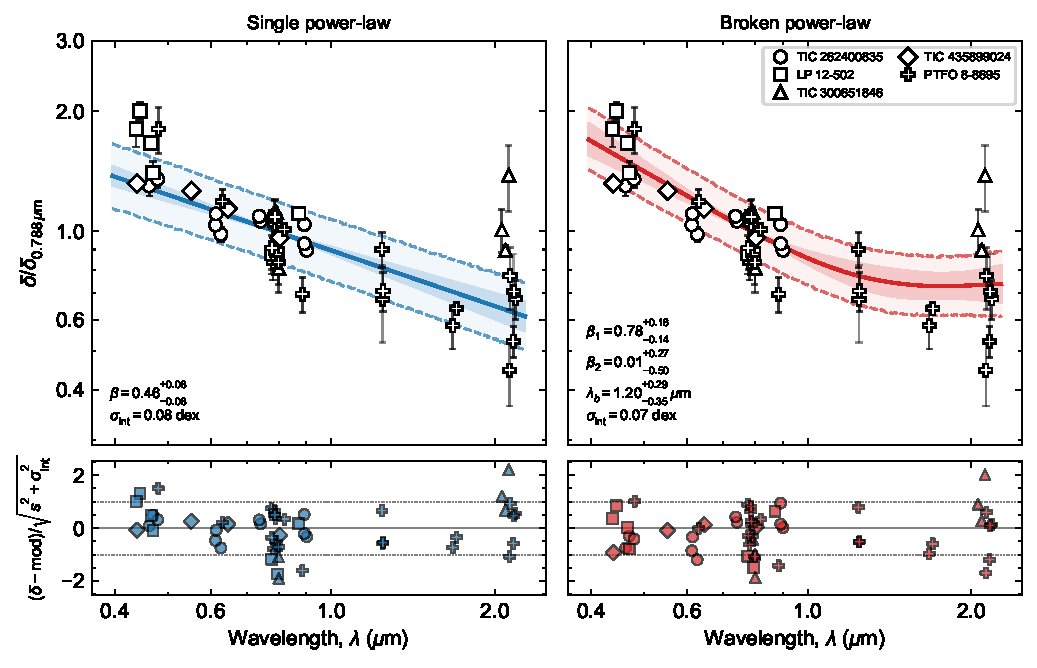
\includegraphics[width=0.99\textwidth]{beta_fits.pdf}
  \vspace{-0.2cm}
  \caption{{\bf Chromaticities of complex periodic variable dips.}
  Markers show the measured dip depth in each bandpass from
  Table~\ref{tab:dipdepths}, with small horizontal jitter added for
  visual clarity.
  The normalization factor $\delta_{0.788\,\mu{\rm m}}$, the depth at
  TESS-band ($\lambda$=0.788\,$\mu$m), is a model-derived quantity per
  combination of star and observing epoch
  (see Section~\ref{subsec:beta}).
  The solid line and inner band are the posterior-median and the 68\%
  confidence interval of the mean $\delta(\lambda)$ relation; the outer band is the 68\%
  predictive interval after additionally accounting for intrinsic
  variability ($\sigma_{\rm int}$).
  Including $\sigma_{\rm int}$, there is a positive preference
  ($\Delta$BIC=\dbicsinglebroken) in favor of the broken power-law.
  Excluding $\sigma_{\rm int}$, there is a strong preference for the
  broken power-law ($\Delta$BIC=\dbicsinglebrokennosig).
  {\it References}: TIC\,262400835, LP\,12-502, and
  TIC\,300651846: this work.
  TIC\,435899024: \citet{Koen2023}.  PTFO\,8-8695: \citet{Yu2015},
  \citet{Onitsuka2017}, \citet{Tanimoto2020}.  }
  \label{fig:beta}
\end{figure*}

We collected literature photometry from observations of CPVs showing
at least one dip that was observed in at least two bandpasses
simultaneously.  Implicitly we also required the dips themselves to be
clearly distinguishable (based on d$f$/d$t$) from spot-induced
modulation, which is also chromatic.  We excluded non-simultaneous
literature datasets even when they carried novel information
(e.g.,~the Spitzer 4.5\,$\mu$m light curve from \citealt{Ciardi2015})
due to the time-variable nature of CPV dip depths.  
Further, we excluded {\it (i)} the TESS-band measurements for
TIC~262400835, due to their low S/N and uncertain crowding correction;
and {\it (ii)} the simultaneous SPECULOOS-South and TESS photometry of
TIC~20178925 from \citet{Gunther2022}, because its ground-based and TESS
dips show different durations, which is inconsistent with the fitting
assumptions we describe below.  

The results are in Table~\ref{tab:dipdepths}.  All told, this data
collection effort yielded 51 dip depth measurements spanning
0.44--2.16\,$\mu$m over five stars and twenty distinct dip epochs.
Half of these measurements are new from this work; the remainder are
from TIC~435899024 \citep{Koen2023} and PTFO~8-8695
\citep{Onitsuka2017,Tanimoto2020}.

We then fitted an extinction law to the dip depths by considering
variants of a model in which
\begin{equation}
  \delta \propto \lambda^{-\beta},
\end{equation}
where $\delta$ is the dip depth and $\beta$ encodes how strongly the
occultation deepens toward the blue.  Positive $\beta$ corresponds to
deeper dips at shorter wavelengths, as expected for extinction by
sub-micron dust; $\beta=0$ is achromatic (gray), as expected for an
optically thick occulter.

Working in logarithmic space, we defined $y_i = \log_{10} \delta_i$,
yielding an uncertainty $\sigma_y \approx |{\rm d}y/{\rm d}{\delta}|
\sigma_\delta $ = $\sigma_{\delta} / (\delta \ln 10)$, for dip index
$i$ at an epoch $e(i)$.  Here we use ``$e(i)$'' to refer to the set of
all multi-wavelength measurements of one dip at a given epoch, and we
use ``$s(i)$'' to refer to the set of all observed dips for any given
star.  We further found it convenient to define $\Lambda_i \equiv
\log_{10}(\lambda_{{\rm eff},i}/ \lambda_0)$, where $\lambda_0$ is an
arbitrary reference wavelength, with a corresponding depth at that
wavelength $\delta_0$.  For convenience, we chose
$\lambda_0$=0.788\,$\mu$m, the effective wavelength of the TESS
bandpass.  We calculated the effective wavelengths of the various
bandpasses using the SVO Filter Profile Service \citep{Rodrigo2020}.
We then considered four model variants:
\begin{align}
  \mu_i &=  c_{e(i)} - \beta \Lambda_i  \quad {\rm (single\ power\ law)}, \label{eq:single} \\
  \mu_i &=  c_{e(i)} - \beta_{s(i)} \Lambda_i  \quad {\rm (per-star\ power\ law)}, \\
  \mu_i &=  c_{e(i)} - \beta_{e(i)} \Lambda_i  \quad {\rm (per-epoch\ power\ law)}, \\
  \mu_i &=  c_{e(i)} - \beta_1 w_i + (\beta_1 - \beta_2) h_i \quad {\rm (broken\ power\ law)}, \label{eq:broken}
\end{align}
where $c_{e(i)} \equiv \log_{10} \delta_{0,e(i)}$ is a fitted reference
depth defined at the reference wavelength $\lambda_0$.  For observations that
have TESS measurements, $c_{e(i)}$ will be near the observed TESS
depth; for those without, $c_{e(i)}$ will be an extrapolation based on
whichever bands were observed.  Finally, in the broken power-law
model, $w_i \equiv \log_{10}(\lambda_{{\rm eff},i}/\lambda_b)$ is the
log-wavelength offset from a free break wavelength $\lambda_b$, and
$h_i \equiv \kappa \ln(1 + e^{w_i/\kappa})$ is a smoothing function
that ensures a continuous gradient in the transition from $\beta_1$
blueward of the break to $\beta_2$ redward of it.  In the broken
power-law model, we take $\lambda_b$ as the reference wavelength for
the per-epoch amplitudes $c_{e(i)}$ rather than $\lambda_0$, and we
set the smoothing scale to $\kappa$=0.01\,dex, since our data do not
constrain it.  Finally, our priors on the fits were $\beta \sim
\mathcal{N}(0,3)$, $c_{e(i)} \sim \mathcal{N}(\langle y_i \rangle,
1)$, and, for the broken power-law model, $\lambda_b/\mu{\rm m} \sim
\mathcal{U}(0.7,1.6)$.  We assumed a Gaussian likelihood, $y_i \sim
\mathcal{N}(\mu_i,\sigma_i)$, where we let $\sigma_i = (s_i^2 +
\sigma_{\rm int}^2)^{1/2}$ optionally add an intrinsic scatter term to
the per-dip uncertainties.  We sampled using PyMC \citep{pymc2023},
and required $\hat{R} < 1.01$ with no divergences as an indicator of
convergence.


\subsubsection{Extinction law results}
\label{subsec:extinction_results}


Figure~\ref{fig:beta} and Table~\ref{tab:fitresults} summarize the
results.  While Figure~\ref{fig:beta} shows the single power-law and
broken-power law results in the $\delta$/$\delta_{0.788\,\mu{\rm
m}}$--$\lambda_{\rm eff}$ plane, we emphasize that the fits are in the
space of $y_i$ vs.~$\Lambda_i$.  The normalization $\delta_{0.788\,\mu{\rm m}}$ is
the model-derived reference depth at the TESS effective wavelength for
each dip epoch in Equations~\ref{eq:single}--\ref{eq:broken}.  To provide a consistent
normalization for visual comparison, we adopted the
$\delta_{0.788\,\mu{\rm m},i}$ values from the ``per-star'' power law
fits, which favors neither of the two displayed models.

All four models agree that the dip depths are chromatic.  
The model-comparison diagnostics also indicate that a single power-law
extinction curve can be improved upon, either by introducing a population-wide
flattening of the extinction toward the near-infrared, or by invoking
epoch-to-epoch or star-to-star variability in the
power-law index.  The detailed interpretation is subject to three key
underlying issues: whether the depth uncertainties $s_i$ can be treated
at face value, how to weigh each model's effective parameter count, and
the degree to which the data can select between the models.

If the dip depth uncertainties were unreliable, then we would want to
incorporate an intrinsic scatter term $\sigma_{\rm int}$, effectively
down-weighting the most precise measurements and weakening our ability
to make model-selection claims on a $\Delta$BIC basis.
We calibrated the reported depth uncertainties as described in
Section~\ref{sec:dipfit}, using the empirical out-of-dip scatter in
each time-series dataset.  The data and fitted model uncertainties (see
Appendix~\ref{app:fit_diagnostics}) suggest that this procedure is
indeed yielding uncertainties that agree with the scatter in the data.
As one example, our refit to the archival literature photometry from
\citet{Onitsuka2017} yielded statistical uncertainties 10-17$\times$
larger than the published values, mirroring the observed scatter.  Our
dip depth uncertainties therefore seem plausible.

Nonetheless, the core drawback of treating our dip depth uncertainties at face value
is that when we do this, the two simple models --- a universal
power-law, and a broken power-law extinction curve --- both
provide poor fits to the data ($\chi^2_\nu$=\singlechirednosig\ and
\brokenchirednosig, respectively).
While inspection of $\chi^2_\nu$ and $\Delta {\rm BIC}$ in
Table~\ref{tab:fitresults} would instead suggest that letting $\beta$
vary on a per-epoch basis is preferred, that choice has serious
drawbacks.  In particular, the ``$\beta$ per-epoch'' model is
pathological for dips observed with only two simultaneous bandpasses,
comprising over half the dataset: this model precludes $\chi^2$ or BIC
from accruing any residual information because it adds free parameters
at the same rate as new data points.  While we explored leave-one-out
style analyses as a possible replacement strategy for counting {\it
effective} free parameters, we ultimately found that with this dataset we were unable to
produce a reliable ranking of this ``per-epoch'' model compared against
the other models.  To some
degree, all four models suffer this ``incidental parameters problem''
\citep{Lancaster2000}, in that every new observation epoch requires
fitting and marginalizing over the depth at the reference wavelength;
the problem is just most severe for the per-epoch model.

In brief, two divergent choices can improve on the single power law:
one could introduce a population-wide break that flattens the
extinction toward the near-infrared, or one could
invoke epoch-to-epoch or star-to-star variability.  Making the
(strong) assumption that the extinction law must be universal,
the preferred model is a broken power-law
with $\beta_1 = \brokenbetaone \pm \brokenbetaoneunc$ blueward of the
break at $\lambda_b = \brokenlambdabreak \pm
\brokenlambdabreakunc$\,$\mu$m, and $\beta_2 = \brokenbetatwo \pm
\brokenbetatwounc$ redward of it.  Intuitively,
this model seems to provide the more plausible explanation for the narrowband
FourStar 2.09\,$\mu$m observations shown in Figure~\ref{fig:fourstar},
which yielded dip depths
\fourstarobsratio$\pm$\fourstarobsratiounc$\times$ the TESS depth,
compared to a predicted ratio from the single-$\beta$ fit of
\fourstarpredratio$\pm$\fourstarpredratiounc\ with $\sint$
(\nunderpredictsigma$\sigma$), or
\fourstarpredrationosig$\pm$\fourstarpredrationosigunc\ without
(\nunderpredictsigmanosig$\sigma$).
With that said, we cannot formally exclude the possibility that
TIC~300651846 is a low-$\beta$ star with no extinction-law break.



\section{Discussion}
\label{sec:disc}

\begin{figure}[!t]
  \centering
  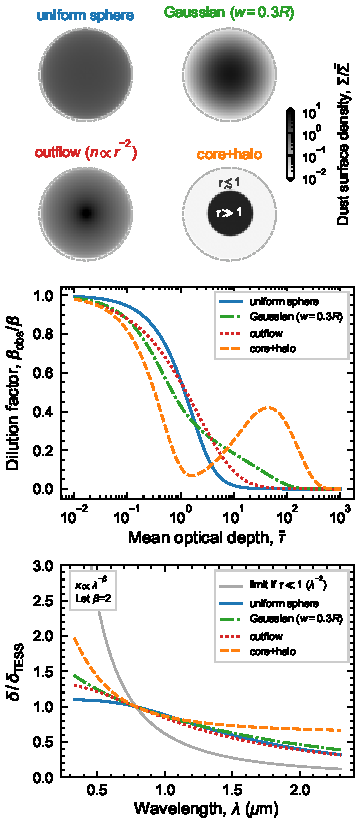
\includegraphics[width=0.44\textwidth]{diluted_transmission_spectrum.pdf}
  \vspace{-0.28cm}
  \caption{{\bf Partial opacity dilutes chromaticity.}
  {\it Top}: surface density maps for four example clump
  profiles.  The ``uniform sphere'' has constant number density; the
  ``core+halo'' (Equation~\ref{eq:corehalo}) has $A_{\rm h}/A_{\rm
  c}$=3.
  {\it Middle}: the factor by which an intrinsic dust opacity
  $\kappa\propto \lambda^{-\beta}$ is diluted into an observed dip
  chromaticity, $\delta \propto \lambda^{-\beta_{\rm obs}}$
  (Equation~\ref{eq:betaobs}).  The mean optical depth, $\bar{\tau}$,
  is averaged over the clump's projected disk.
  At fixed $R$ and $\kappa$, profiles with equal
  $\bar{\tau}$ contain equal dust mass.
  {\it Bottom}: example spectra for $\beta$=2; the
  smooth profiles set $\bar{\tau}_{\rm TESS}$=3, and the core+halo
  profile sets $\tau_{\rm h}$=0.1 at 1.2\,$\mu$m.  Only the bimodal
  core+halo profile matches Figure~\ref{fig:beta}.
  }
  \label{fig:betadilution}
\end{figure}


\subsection{An opaque core and an optically thin halo of dusty plasma}
\label{sec:dustyplasma}

It is tempting to read Table~\ref{tab:fitresults} and
Figure~\ref{fig:beta} as measurements of
the dust opacity law, $\kappa(\lambda)$, whose shape is connected to
the size distribution and composition of the dust grains.  While
$\delta(\lambda)$ and $\kappa(\lambda)$ are
related, there is a nuance: the mapping is only direct
when the occulting material is optically thin.  Nothing about the data
guarantees that we are in this regime.  Consider an absorbing
clump of material occulting a uniform stellar disk of area $A_\star$.
The dip depth $\delta$ is
\begin{equation}
  \delta(\lambda) = \frac{1}{A_\star}
  \int \left[ 1 - e^{-\kappa \Sigma} \right] {\rm d}A,
  \label{eq:depthintegral}
\end{equation}
where $\Sigma$ is the surface density of the dust, $\kappa$ is the
opacity (and only wavelength-dependent term), and the integral is over
the dust clump's area.  Approximating
$\kappa(\lambda) \propto \lambda^{-\beta}$ in the optical and
near-infrared, one can show that the {\it observed} slope $\beta_{\rm obs}$ from
$\delta(\lambda)$ in Figure~\ref{fig:beta} is related to the
{\it underlying} dust opacity law's $\beta$ through
\begin{equation}
  \beta_{\rm obs} \equiv
  -\frac{{\rm d} \ln \delta}{{\rm d} \ln \lambda}
  = \beta \, \frac{{\rm d} \ln \delta}{{\rm d} \ln \kappa}.
  \label{eq:betaobs}
\end{equation}
The derivative on the right-hand side is a ``dilution factor'' which lies between
0 and 1 for any surface density distribution.  The observed dip-depth
$\beta_{\rm obs}$ of Table~\ref{tab:fitresults} and
Section~\ref{subsec:beta} therefore provides only a lower bound on the
dust opacity's $\beta$, with the two related by
Equation~\ref{eq:betaobs}. 

% NOTE:
% each Σ scale in the distribution produces one bump centered at τ ~ 1
% for that scale; the bimodal surface density distribution, with
% well-separated scales, gives two bumps with a valley between.
%
% NOTE also:
% \bar{\tau} \equiv (\pi R^2)^{-1}\int \kappa\Sigma\,{\rm d}A
%   = \kappa M/(\pi R^2)

Figure~\ref{fig:betadilution} quantifies this damping for
representative surface-density profiles and mean optical depths.  
Note that while the ``uniform sphere'' profile has $\Sigma(r) \propto
(R^2 -r^2)^{1/2}$, this is not visible in the top panels due to the
color stretch.
The Gaussian has width $w$ such that $\Sigma(r) \propto \exp(-r^2 / (2 w^2)$.
The
middle panel shows that for the smooth profiles, by a mean optical
depth $\bar{\tau}$$\approx$1
the observed slope falls to 40--60\% of the intrinsic slope, and by
$\bar{\tau}$$\approx$3 to 20--30\%.
The lower panel gives example vertical slices from the middle,
setting
$\bar{\tau}$$=$3 for the smooth profiles and exploring the impact of
dilution on a ``steep''
$\beta$=2 intrinsic grain opacity.
All models flatten the extinction curve.
However, even after accounting for this dilution, comparison with
Figure~\ref{fig:beta} shows that the smooth profiles provide
a poor fit to the data: their blue dips are not deep enough, and
their $K$-band dips are too shallow.

If dust provides the opacity,
the simplest physical interpretation of a
broken power-law in $\delta(\lambda)$ is to therefore invoke a {\it bimodal}
surface density distribution: an opaque core of projected area
$A_c$ ($\tau \gg 1$ out through $K$ band) surrounded by an optically
thin halo of area $A_h$ and depth $\tau_h(\lambda)$.  Such a 
distribution yields
\begin{equation}
  \delta(\lambda) \approx \frac{A_c}{A_\star}
  + \frac{A_h}{A_\star} \left[ 1 - e^{-\tau_h(\lambda)} \right],
  \label{eq:corehalo}
\end{equation}
such that the infrared depths sit on the core's gray floor while the
optical depths are dominated by the halo's chromatic term, with the
break falling near where the two terms are comparable.
The ``core+halo'' curve in the lower panel of
Figure~\ref{fig:betadilution} shows a toy example with
$A_{\rm h}/A_{\rm c}$=3 and $\tau_{\rm h}(1.2\,\mu{\rm m})$=0.1: the
same $\beta$=2 opacity law that the smooth profiles flatten into a
gray curve instead yields a broken power law resembling the data.
A brute-force exploration of the parameter space indicates 
an allowed parameter range of 
$1 \lesssim A_{\rm h}/A_{\rm c} \lesssim 30$, $10^{-4}\lesssim
\tau_{\rm h}\lesssim 0.3$ at 1.2\,$\mu$m, and $1\lesssim \beta
\lesssim 4$, where the upper bound on $\beta$ is the
Rayleigh-scattering limit.
This range of $\beta$ excludes the possibility of a population
dominated by mm to cm-sized solids, but is otherwise 
consistent with a wide range of dust compositions and size
distributions.



\subsection{Where do the dust and plasma come from?}
\label{sec:origin}

\begin{figure}[!t]
  \centering
  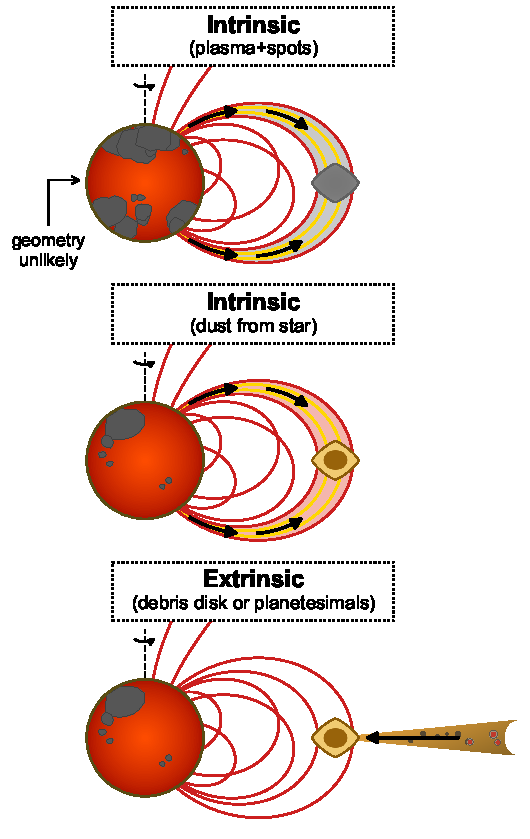
\includegraphics[width=0.48\textwidth]{cgcd_cartoons_b_mixed_geom.pdf}
  \vspace{-0.4cm}
  \caption{{\bf Origin scenarios for the opaque occulting material.}
  {\it Top}: corotating plasma clumps plus high starspot filling
  factor and no dust.  
  {\it Center}: Dust condensing from magnetically confined stellar
  plasma.  
  {\it Bottom}: Dust captured from an extrinsic reservoir (debris disk
  or undetected planetesimals).
  The dust-free scenario is disfavored; the lower two remain possible,
  and differ in where the dust originates.
  At least some starspots are present in all scenarios.
  The stars must have ``centrifugal'' magnetospheres with
  magnetospheric radii $R_{\rm m}$ exceeding their corotation radii
  $R_{\rm c}$; the clumps remain long-lived only between the two
  extremes.
  }
  \label{fig:cartoons}
\end{figure}

Where does the occulting material responsible for CPV dips come
from?  Figure~\ref{fig:cartoons} sketches three possible scenarios.
Starspots are present in every scenario since CPVs are young, magnetically active, and
show smooth rotational modulation over which the dip signals are
superposed.  
While dark facular networks could also be present \citep{Shapiro2026}, they
are relevant only in that they could influence this smooth
variability.  

In scenario {\it (i)}, the plasma clumps condense out from the star
without any dust being present \citep[e.g.][]{Daley-Yates2024}, and a
very specific starspot geometry is also required.
In this scenario, the chromaticity of the dips needs to somehow be
provided by the plasma, the spots, or a combination thereof.
However the plasma cannot do it alone: neither H$^-$ opacity nor
hydrogen bound-free opacity provide the correct functional forms.
Instead, the most likely opacity source would be
scattering from the free electrons (Thomson scattering); this would
need to be
combined with the ``transit light source effect'' \citep{Rackham2018}
in which unocculted spots outside the transit chord provided the
apparent chromaticity.
Exploring such models however shows that the requisite
spot-covering fractions $f$ are in the range of 70--90\% of the stellar area.
CPVs often require $R/R_\star$$\gtrsim$0.1.
The geometric probability of having clear transit chords for the entire 
chromatic ensemble of observed CPV dip is sufficiently low to be ruled
out.
Separate arguments against this scenario include the lack of response
in the light curves to changes in circumstellar emission 
(Section~\ref{subsec:mage_interpret}), and the 
{\bf Facundo(?): the evidence from TSPEC spectra for starspot covering
fractions $f$$\lesssim$XX\% in LP~12-502}.

While we disfavor Scenario~{\it (i)}, the data remain compatible
with both Scenarios~{\it (ii)} and~{\it (iii)}.
In either dust scenario, the dust becomes collisionally charged
\citep{Sanderson2023},
enabling it to remain magnetically confined \citep{Daley-Yates2026}.
The two scenarios may differ in their expected extent of mixing
between the gas and dust, as well as in the composition of the grains
themselves.
Either dust origin channel would be yielding new information:
in Scenario~{\it (ii)} we would learn that young M dwarfs condense out dust,
similar perhaps to how this happens in the atmospheres of AGB stars
\citep{Hofner2018}.
In Scenario~{\it (iii)} we would gain a new way of identifying and
studying the detritus of planet formation.


\subsection{Continued relevance of PTFO\,8-8695}
\label{sec:ptfo}

The saga of PTFO\,8-8695 (CVSO 30), whose data appear in
Figure~\ref{fig:beta}, provides unique connections to the current
CPV literature.  To recap: \citet{vanEyken2012} identified a hot
Jupiter candidate in Orion; \citet{Barnes2013} and \citet{Kamiaka2015}
subsequently argued that its orbit was nodally precessing, and
\citet{Johns-Krull2016} found that the source showed
sinusoidal-in-time H$\alpha$ emission at circumstellar velocities.
Photometric follow-up found the planet candidate's orbital period to
stay fixed, but that the ephemeris jumped around in orbital phase and
split into multiple dips per cycle
\citep{Ciardi2015,Yu2015,Raetz2016,Onitsuka2017,Tanimoto2020}.
\citet{Bouma2020} used TESS and Gaia to argue that the system shows
multiple indicators for being an intermediate-separation (multiple~AU)
binary, one component of which shows an ordinary rotation signal, and
the other component being a complex periodic variable.  While this
interpretation may not be uniformly accepted \citep{Grosson2021},
further photometric follow-up by \citet{Bischoff2022} has been broadly
consistent.

The characterization of PTFO 8-8695 provided photometric and
spectroscopic details that have been remarkably prescient for
understanding CPVs.  Spectroscopically, \citet{Johns-Krull2016} showed
evidence for Balmer variability similar to that seen for TIC~141146667
and TIC~300651846, and consistent with the idea of bound circumstellar
plasma being present.  Photometrically, \citet{Tanimoto2020} monitored
the source for five years in optical and infrared bands, and observed
a break in the chromaticity of this system's dip depths going out to
$K$-band similar to that reported in this work.  One of their proposed
resolutions was the scenario of an opaque dust core with an optically
thin dust halo---and this is exactly the scenario that we favor from
Section~\ref{subsec:extinction_results}.  The Spitzer 4.5\,$\mu$m
light curve observed by \citet{Ciardi2015} showing a 0.5\% deep dip in
2012 remains a unique dataset, and it remains the only information we
have about the chromaticities of any CPV dips redward of $K$-band.

\subsection{The chromaticity differs from analog magnetic rotators}

Massive magnetic B stars are the only class of star known to exhibit
similar light curves to CPVs.  The prototype, $\sigma$ Ori~E, has a
long history \citep[e.g.][]{Landstreet1978,Townsend2005b,Oksala2015},
but the summary is that it hosts a centrifugally supported
magnetosphere in which a long-lived ``pinched'' plasma torus
\citep{Townsend2008} produces photometric eclipses and
sinusoidal-in-time spectroscopic emission.  \citet{Bouma2024} argued
that the additional step to produce ``complex'' light curves comes
from magnetic topology, on the basis that the few $\sigma$ Ori~E
analogs showing complex light curves also show (rare) evidence from
Zeeman Doppler imaging for non-dipolar magnetic fields.  The analogy
extends to the radio: $\sigma$ Ori~E shows rotationally modulated
gyrosynchrotron emission from its corotating magnetosphere
\citep{Leto2012}, and polarized, variable radio emission has now been
reported for two CPVs, DG~CVn \citep{Kaur2025} and TIC~146539195
\citep{Kaur2024,Curiel2026}.

While physical analogies can be drawn, the chromaticities of the
$\sigma$ Ori~E analog eclipses are different from what is seen for
CPVs.  \citet{Hesser1977} and \citet{Oksala2007} provided photometry
that showed near-gray chromaticity in $vby$, with a slight depth
decrease in $v$ relative to $y$, and a major depth increase in $u$.
This behavior mirrors the hydrogen bound-free opacity curve as a
function of wavelength \citep{Gray2008}: the Balmer break at
3646\,\AA\ captures the $u$ band, while $vby$ would have a slight
decrease before the break.  This is consistent with the opacity in the
$\sigma$ Ori~E analogs coming purely from trapped hydrogen.  While
$u$-band photometry of CPVs does not exist, their behavior in the
$griz$ optical bands is inconsistent with the predictions of the
bound-free opacity.

% \subsection{What data would help?}
% \label{subsec:whatdata}
% 
% Actual Transmission spectroscopy.
% 
% Simultaneous in the optical, and the near+mid IR.
% 
% Also, UV, simultaneous with at least the optical.  Maybe w/ other
% wavelengths too.


\section{Conclusions}
\label{sec:conc}

CPVs show a combination of smooth, rotationally-induced modulation,
along with sharp dips induced by the transits of magnetically bound
circumstellar material.  The occulting material must be circumstellar
because of how quickly it causes the broadband flux to change,
and magnetically bound because of its
synchronicity with the stellar rotation
period 
and its sensitivity to flaring 
\citep{Stauffer2017,Bouma2024}.  The composition of the
circumstellar material could, a priori, be gas, dust, or a combination
thereof.  In this work we find that while circumstellar gas is
conspicuously present, dust seems to provide the opacity source
responsible for the dips.

Gas is conspicuously present {\it (i)} because of sinusoidal-in-time
Balmer emission out of transit, and {\it (ii)} because of Balmer line
extinction during transit.  Plasma clump emissivity out of transit was
first seen in CPVs for TIC~141146667 \citep[$n_{\rm
H}$$\approx$1$\times$10$^{11}$\,cm$^{-3}$;][]{Bouma2025}.  Observing
TIC~300651846 and LP~12-502 at comparable sensitivity gave a
detection of bound emitting
circumstellar plasma for TIC~300651846 ($n_{\rm
H}$$\approx$3--8$\times$10$^{11}$\,cm$^{-3}$;
Section~\ref{subsec:mage_interpret}), and upper limits for LP~12-502
($n_{\rm H}$\,$\lesssim$\,5$\times$$10^{10}$\,cm$^{-3}$;
Appendix~\ref{app:keck_ootspec}).  The quoted range for TIC~300651846
comes from the six-fold variation in H$\alpha$ clump luminosity seen
night-to-night, implying a number density variation of
2.5$\times$.
This large spectroscopic change was accompanied by no
discernable changes in simultaneous TESS data.  The lack of
correlation between light curve morphology and circumstellar plasma
number density suggests that gas is not responsible for the sharp
dips, leaving dust as the only viable culprit.

The gas and dust appear spatially associated: both the
high-resolution (Figures~\ref{fig:mage} and~\ref{fig:mike}) and
low-resolution (Figure~\ref{fig:dbsp}) time-series spectra show
H$\alpha$ transits occurring simultaneously or near-simultaneously
with broadband flux transits.
We did observe departures from strict simultaneity through
repeatable transit timing offsets for two stars: for TIC~300651846 the deepest
H$\alpha$ minimum preceded the deepest broadband flux local minimum by
$\approx$25\,minutes on all five nights from January~2025; for
LP~12-502 the offset was $\approx$50\,minutes late over both nights in
November~2023.

Chromaticities from broadband photometry currently provide the best
information about the dust composition.  We compiled our new
observations with the literature and fitted four variants of a $\delta
\propto \lambda^{-\beta}$ extinction curve: a single power-law, a
broken double power-law, a power-law that let $\beta$ vary per-star,
and a power-law that let $\beta$ vary per epoch.  The results, shown
in Table~\ref{tab:fitresults} and Figure~\ref{fig:beta}, show that the
two simpler models (single and broken power-law) both yield
poor fits ($\chired$$\gg$1).  This suggests either that there is
star-to-star or epoch-to-epoch variability in the extinction law
(produced for instance by an inhomogeneous and evolving dust population),
or that there is an unknown source of intrinsic scatter that requires
inflating the observed dip depth uncertainties.  Our analysis also
highlighted the challenge of formal BIC-based model
comparison for these data: the epoch-to-epoch depth variability of
CPVs implies that we must marginalize over a transit depth at a
reference wavelength for each observing epoch, which negates the
statistical value of two-band epochs that lack TESS data.

Our results therefore leave an open degeneracy: one can 
improve on the single power law extinction curve by either
introducing a broken power-law, or by invoking epoch-to-epoch or
star-to-star variability in the power-law index.  While these ideas
are not mutually exclusive, they cannot be distinguished with the current
data because the near-infrared data for TIC~300651846 and PTFO~8-8695
come with only a single optical anchor point each.  Nonetheless, 
a broken power-law seems to provide the
simplest explanation for the depth of CPV dips in the infrared
(see~Figure~\ref{fig:fourstar}, and \citealt{Ciardi2015}).  Our fits
for such a model yielded $\beta_1 = \brokenbetaone \pm
\brokenbetaoneunc$ blueward of the break at $\lambda_b =
\brokenlambdabreak \pm \brokenlambdabreakunc$\,$\mu$m, and $\beta_2 =
\brokenbetatwo \pm \brokenbetatwounc$ redward of it.

The break, rather than the slopes, carries most of the physical
information
(Sections~\ref{sec:dustyplasma} and~\ref{sec:origin}).
The {\it observed} optical chromaticity $\beta_1$ provides
a lower bound on the {\it intrinsic} spectral index of the dust
opacity: for $\kappa \propto \lambda^{-\beta}$ we infer $1<\beta<4$.
This excludes a dust population dominated by
mm to cm-sized solids, but is otherwise consistent with a wide range of
dust compositions and size distributions.
The break itself can be produced
by a bimodal dust surface
density distribution: an opaque core surrounded by an optically thin
halo.  We find that such a model can reproduce the data for halo to
core area ratios $1 \lesssim A_{\rm h}/A_{\rm c} \lesssim 30$ and 
halo optical depths $10^{-4}\lesssim \tau_{\rm h}\lesssim 0.3$ at
1.2\,$\mu$m.

While all approximations are wrong, some are useful.  The core+halo
picture is useful in that it reproduces the observed extinction curve
with a minimum of ingredients; it is surely also wrong in its details.
Spectral features of the occulting dust and gas, particularly in the
ultraviolet and infrared where data are currently
lacking, offer one area for future work.



\begin{acknowledgements}
  \newline
  L.G.B. gratefully acknowledges support from the Carnegie Fellowship
  and the Heising-Simons 51 Pegasi~b Fellowship during the data
  collection phase of this project.
	J.G.M. gratefully acknowledges support from the Heising-Simons Foundation and
	the Pappalardo family through the MIT Pappalardo Fellowship in Physics.
  We thank the staff of Magellan, Keck, and Palomar
  Observatories, including the telescope operators and instrument
  specialists, for their support of the observations presented in this
  work; we also thank Eric Persson for assistance with FourStar
  observation planning.
  This work also used data from TESS \citep{TESS2min}.
  % via https://heasarc.gsfc.nasa.gov/docs/tess/approved-programs.html
  The 2-minute cadence observations used in this work were proposed by
  the guest observer (G) and director's discretionary time (DDT)
  programs listed below; we used light curves from SPOC
  \citep{Jenkins2016}, TARS \citep{Boyle2026}, and unpopular
  \citep{Hattori2022}.
  % 300651846 S98
  {\it TIC~300651846:}
  % 300651846 S87 + S88 G07140;G07036;G07103
  G07140 (A.~Boyle), G07036 (T.~Wainer), G07103 (L.~Bouma);
  G08046 (M.~Battley), G08137 (A.~Feinstein).
  % DG CVn S50
  {\it DG~CVn:}
  % G04212;G04132;G04211;G04188;G04039;G04191;20SECONDTARGET
  G04212 (R.~Paudel), G04132 (W.~Howard), G04211 (F.~Marocco), G04188
  (M.~Silverstein), G04039 (J.~Davenport), G04191 (J.~Burt).
  % LP 12-502 / 402980664 s58
  {\it LP~12-502:}
  G05106 (E.~Gillen), G05152 (R.~Cloutier), 
  % LP 12-502 s73
  G06030 (L.~Bouma), G06120 (E.~Gillen),
  % LP 12-502 s86
  G07089 (E.~Gillen), G07103 (L.~Bouma).
  {\it TIC 262400835:}
  DDT028 (L.~Bouma).
  Funding for the TESS mission is provided by NASA's Science Mission
  directorate.
  The HIRES data were obtained at the Keck Observatory.
  We recognize the importance that the summit of Maunakea has always
  had within the indigenous Hawaiian community, and we are grateful
  for the opportunity to conduct observations from this mountain.
	This work makes use of observations from the Tierras Observatory, which is
	supported by the National Science Foundation under Award No. AST-2308043.
	Tierras is located within the Fred Lawrence Whipple Observatory; we thank all
	the staff there who help maintain this facility.
  This article is also based on observations made with the MuSCAT2
  instrument, developed by ABC, at Telescopio Carlos Sánchez operated
  on the island of Tenerife by the IAC in the Spanish Observatorio del
  Teide.  This work is partly supported by JSPS KAKENHI Grant Numbers
  JP24H00017, JP25K24620, JP26H01402, JP24K00689, JP25K17450,
  JP26K00755 and JP26K17193.
  We also acknowledge financial support from the Agencia Estatal de
  Investigaci\'on of the Ministerio de Ciencia e Innovaci\'on
  MCIN/AEI/10.13039/501100011033 and the ERDF ``A way of making
  Europe''
  through projects PID2021-125627OB-C32 and PID2024-158486OB-C32. This
  work is supported by the ERC Grant (ERC Advanced Grant SPEAR, GA
  101200674), funded by the European Union.  Views and opinions
  expressed are however those of the author(s) only and do not
  necessarily reflect those of the European Union or the  European
  Research Council Executive Agency (ERCEA). Neither the European
  Union nor the granting authority can be held responsible for them.
\end{acknowledgements}

{\it \large Contributions}: 
LGB led the inception, design, execution, and interpretation of the
project.  Data were acquired and reduced by JHL, KI, NN, and AK
(MuSCAT1); EP, FM (MuSCAT2); JGM, PT, DC (Tierras); AB
(KeplerCam); FPP (TSPEC); and LGB (MIKE, MagE, FourStar, HIRES, DBSP, TSPEC).
Observations by JSS (FourStar) and ASC (HIRES), and reduction
assistance by HI and AWH (HIRES) enabled the work.  AM
helped plan and interpret the FourStar observations.  Finally, FPP, LAH, AJW,
JJS, MMJ, JAV, and DRC contributed to the interpretation of the
results, and all authors reviewed the manuscript.

\facilities{
  Magellan:Baade,
  Magellan:Clay,
  Keck:I,
  Hale,
  OAO:1.88m,
  Sanchez,
  FLWO:Tierras,
  FLWO:1.2m,
  Gaia,
  TESS,
	2MASS,
	SDSS.
}

\software{
  astroariadne \citep{Vines2022},
  astropy (\citealt{astropy:2013,astropy:2018,astropy:2022}),
  carpy \citep{Kelson2000,Kelson2003},
	DBSP\_DRP \citep{dbsp_drp:zenodo},
	dustmaps \citep{2018JOSS....3..695M},
  matplotlib \citep{matplotlib},
  numpy \citep{numpy},
  PyMC \citep{pymc2023},
	PypeIt \citep{dbsp_drp:joss},
  scipy \citep{scipy}.
}




%%%%%%%%%%%%%%%%%%%%%%%%%%%%%%%%%%%%%%%%%%%%%%%%%%%%%%%%%%%%%%%%%%%%%%%%%%%%%%%
%%%%%%%%%%%%%%%%%%%%%%%%%%%%%%%%%%%%%%%%%%%%%%%%%%%%%%%%%%%%%%%%%%%%%%%%%%%%%%%

\appendix
%
\section{Spectroscopy of CPVs Outside the Narrow Flux Dips}
\label{app:ootspec}

In the main text we focus on photometric and spectroscopic signatures
of the circumstellar material present around CPVs.  However, due to
the long-term unpredictability in CPV light curve morphology, some
nights yielded coverage of only spot-induced or flare-induced
broadband flux variability without providing any
evidence---spectroscopic or photometric---for bound circumstellar
material.  We describe the results of those observations below.

\subsection{Keck/HIRES}
\label{app:keck_ootspec}

Figure~\ref{fig:hires} summarizes TESS and HIRES data for LP~12-502 on
the nights of 23~November 2023, 3~December 2024, and 10~December 2024.
The static spectra exhibit Balmer series emission up to
$n$=15$\rightarrow$2, strong chromospheric emission in the
\ion{Ca}{2}~H\&K lines, and the expected forest of molecular
absorption lines for a non-accreting (``weak-lined'') pre-main
sequence M4.5Ve dwarf.

The HIRES spectra show flare-induced variability over
all three nights.  The most direct indicator for this variability is
in chromospheric emission lines; excess emission appears during the
variable epochs while the redder orders, including the
order-normalized continuum, appear stable.  This spectral variability
is temporally coincident with elevated TESS flux levels
(Figure~\ref{fig:hires}), and is symmetric in the blue and red wings
of the Balmer lines in the time-dynamic spectra, consistent with
electric field-induced pressure broadening \citep{Kowalski2017}.  This
structure is mirrored across numerous chromospheric lines, including
the entire Balmer series, the \ion{Ca}{2}~H\&K lines,
\ion{Ca}{1}\,4226, \ion{He}{1}\,4026, \ion{He}{1}\,4471, the Na
doublet, and the Mg triplet.  The flaring epochs also coincide
with the excitation of at least a dozen \ion{Fe}{1} lines spanning
3820\,\AA--4050\,\AA \citep{NIST_ASD}.  These lines are not present in the quiescent
spectra; they appear in emission with
$\Delta\lambda$$\approx$0.2\,\AA\ 
over the few-hour duration for which the other flare diagnostics are
also present.  This is consistent with established phenomenology for M
dwarf flares \citep{Fuhrmeister2008}.

% re: iron lines, cf
% https://docs.google.com/spreadsheets/d/18ADpjTs8v_zp22vRA5i7o6JrJvtaq8PYVZeiCXbQo-k/edit?usp=sharing
%
% full details in 20240708_j531_LP12-502_metal_emission_line_analysis.txt

While the HIRES spectra and photometry of LP~12-502 presented abundant
evidence for flare-induced variability, no variability could be
clearly associated with any bound circumstellar hydrogen.
Nonetheless, the same calculation as in
Section~\ref{subsec:mage_interpret}, enables a conversion of this 
non-detection of H$\alpha$ emission  to an upper limit on the number
density of bound circumstellar plasma.
% via /Users/luke/Dropbox/proj/hotcold/drivers/calc_number_density_constraint_from_ha_emission.py
For LP~12-502, $L_\star$=0.011$\pm$0.001\,L$_\odot$,
$R_\star$=0.37$\pm$0.01 \citep{Bouma2024}, and we measure a mean
stellar H$\alpha$ EW and scatter of $0.22 \pm 0.02$\,\AA.  The implied
stellar H$\alpha$ line luminosity is
$\approx$3.0$\times$10$^{26}$\,erg\,s$^{-1}$, two orders of magnitude
lower than TIC~300651846.
We derive an upper limit on the equivalent width of any excess
H$\alpha$ by injecting synthetic emission into the spectra shown in
Figure~\ref{fig:hires}.
This process indicated that we would have been sensitive to 
circumstellar H$\alpha$ emission with EW $\gtrsim$ 10 m\AA.
As a result, we can rule out plasma clumps with number density $n_{\rm
H} \gtrsim 5 \times 10^{10}$\,cm$^{-3}$, or assuming
$r$$\approx$0.1\,$R_\star$, any clumps with $M_{\rm
gas}$$\gtrsim$6$\times$10$^{15}$\,g.
This limit on the clump hydrogen number density is an order of
magnitude lower than the densities observed for TIC~141146667
($\approx$1$\times$10$^{11}$\,cm$^{-3}$; \citealt{Bouma2025}) and
TIC~300651846 (3--8$\times$10$^{11}$\,cm$^{-3}$;
Section~\ref{subsec:mage_interpret}).

\begin{figure*}[!t]
  \centering
  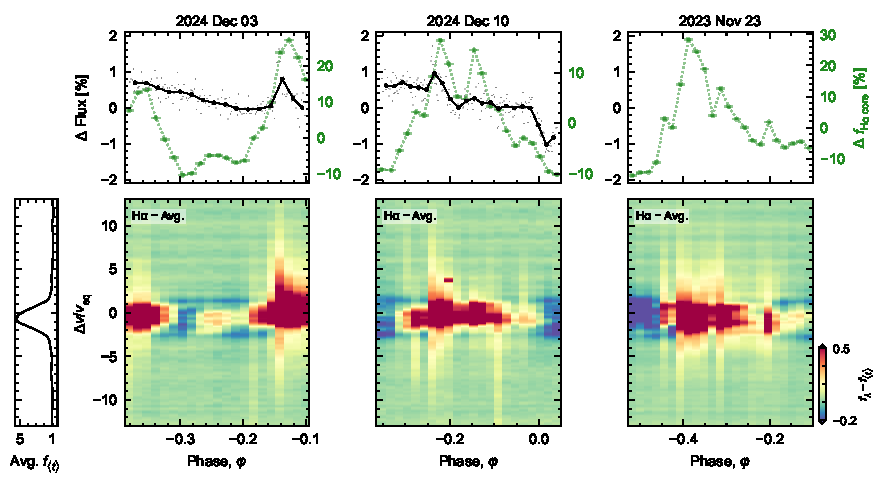
\includegraphics[width=0.8\textwidth]{hires_lp12502_mosaic.pdf}
  \vspace{-0.2cm}
  \caption{{\bf Flare-induced variability of LP~12-502 viewed through
  Keck/HIRES and TESS}.  The lower left panel shows the time-average
  H$\alpha$ profile on 3~December 2024.  The successive columns show
  the time-dynamic mean-subtracted H$\alpha$ profiles on the bottom.
  On top, simultaneous TESS flux measurements are in black, with the
  median-normalized H$\alpha$ line flux at $|v/v_{\rm eq}|<1$ in
  green.  The lack of (bound) circumstellar emission yields an upper
  limit on the number density of any plasma clumps, discussed in the
  text.}
  \label{fig:hires}
\end{figure*}


\subsection{Hale/DBSP}
\label{app:dbsp_ootspec}

Figure~\ref{fig:dbsp_supp} shows three near-adjacent nights observing
LP~12-502 with Hale/DBSP.  Figure~\ref{fig:dbsp_Nov2024}
gives a complete visualization of the TESS flux and DBSP H$\alpha$~EW
behavior over the five adjacent nights in November~2024, folded on the
18.56\,hour period.  While LP~12-502 exhibited extreme variability
from 2019--2023, showing four to eight sharp flux dips per cycle, it
displayed only one or two sharp flux dips from May to December~2024
(TESS Sectors 78--86).  A movie showing the star's TESS light curve
from 2019--2025 is
\href{https://lgbouma.com/movies/LP_12-502_20250218.mp4}{{\bf
available online}}.  In our November~2024 DBSP run, flare-induced
variability played a significant role in modulating the
H$\alpha$ equivalent width measurements, and only two of the five
nights (discussed in the main text) overlapped with the complex flux
dips that define the CPV class.

\begin{figure*}[!t]
  \centering
  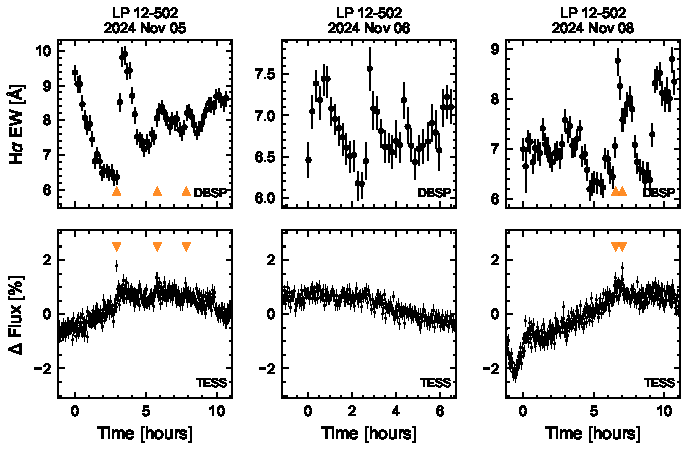
\includegraphics[width=0.75\textwidth]{DBSP_HAlpha_mosaic_supp.pdf}
  \vspace{-0.2cm}
  \caption{{\bf Hale/DBSP H$\alpha$ equivalent widths (EWs)
  vs.~simultaneous TESS photometry during ``non-complex'' windows.}
  Panels are as in Figure~\ref{fig:dbsp}, but for the three nights
  with only flare- and spot-induced variability.  On Nov~5,
  flare-induced local maxima occur at $t$=3.5, 6, and 8~hours; on
  Nov~6 a similar maximum occurs at $t$=2.6\,hours; and on Nov~8, at
  $t$$\approx$6.5\,hours.  The Nov~8 DBSP observations began just
  after the end of a sharp ``complex'' flux dip.  }
  \label{fig:dbsp_supp}
\end{figure*}

\begin{figure*}[!t]
  \centering
  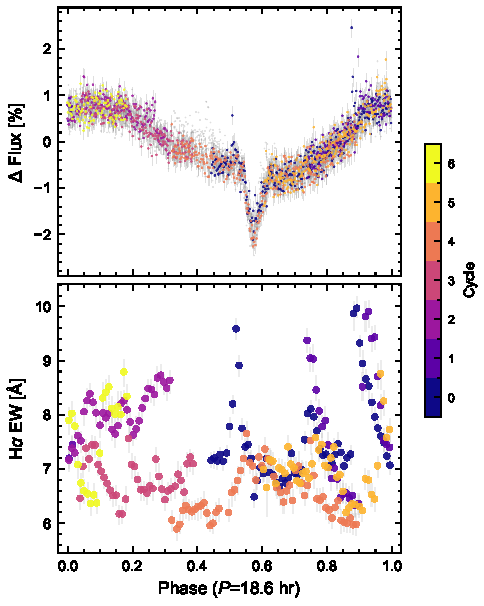
\includegraphics[width=0.48\textwidth]{LP12-502_Nov2024_dbsp_vs_tess.pdf}
  \vspace{-0.2cm}
  \caption{{\bf LP~12-502 Hale/DBSP H$\alpha$ equivalent widths (EWs)
  vs.~simultaneous TESS photometry from 4~November 2024 to 8~November
  2024.} Points are colored by their orbital cycle number relative to
  the first 18.56\,hour period.  Simultaneous TESS measurements using
  the main colormap; TESS data in the 4~November to 8~November
  baseline that were not covered {\it simultaneously} by DBSP due to
  the day-night cycle are shown in gray.
  }
  \label{fig:dbsp_Nov2024}
\end{figure*}


\section{Time-Series Photometry Fitting Diagnostics}
\label{app:fit_diagnostics}

Figures~\ref{fig:dipfit1} and~\ref{fig:dipfit2} show the results from
our photometry fitting routine, which forms the basis for the
chromaticity analysis in Section~\ref{subsec:beta}.

\begin{figure*}[!tp]
  \centering
  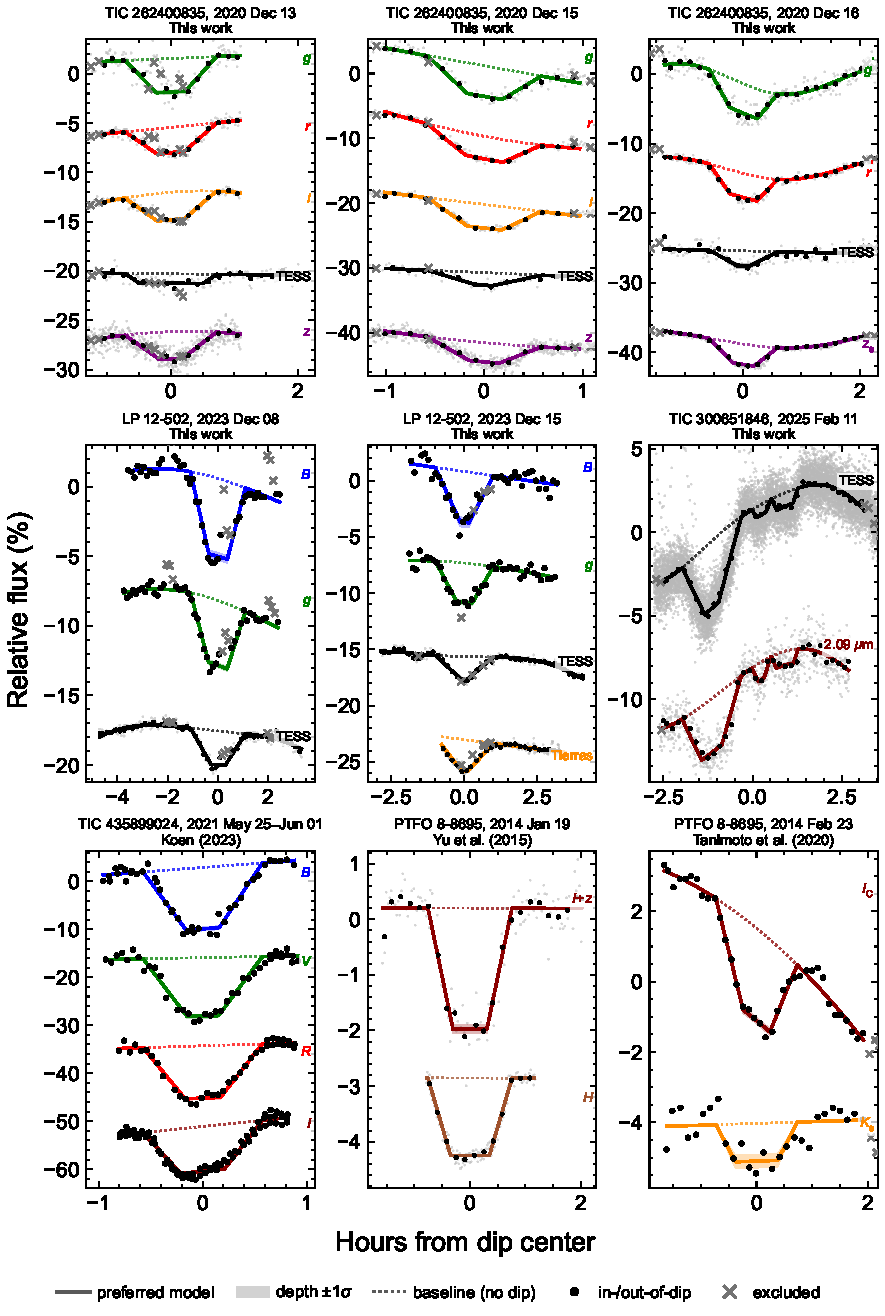
\includegraphics[width=0.8\textwidth]{dip_fit_mosaic_1.pdf}
  \vspace{-0.2cm}
  \caption{{\bf Trapezoidal fits to multi-band photometry of CPVs
  (part 1/2).} Data from TIC\,262400835, LP\,12-502, and
  TIC\,300651846 and new to this work.  We digitally transcribed the
  measurements from TIC\,435899024 \citep{Koen2023} and PTFO\,8-8695
  \citep{Yu2015,Tanimoto2020}.  Dip depth uncertainties
  ($\pm$1-$\sigma$) are shown in the underplotted contours.}
  \label{fig:dipfit1}
\end{figure*}

\begin{figure*}[!tp]
  \centering
  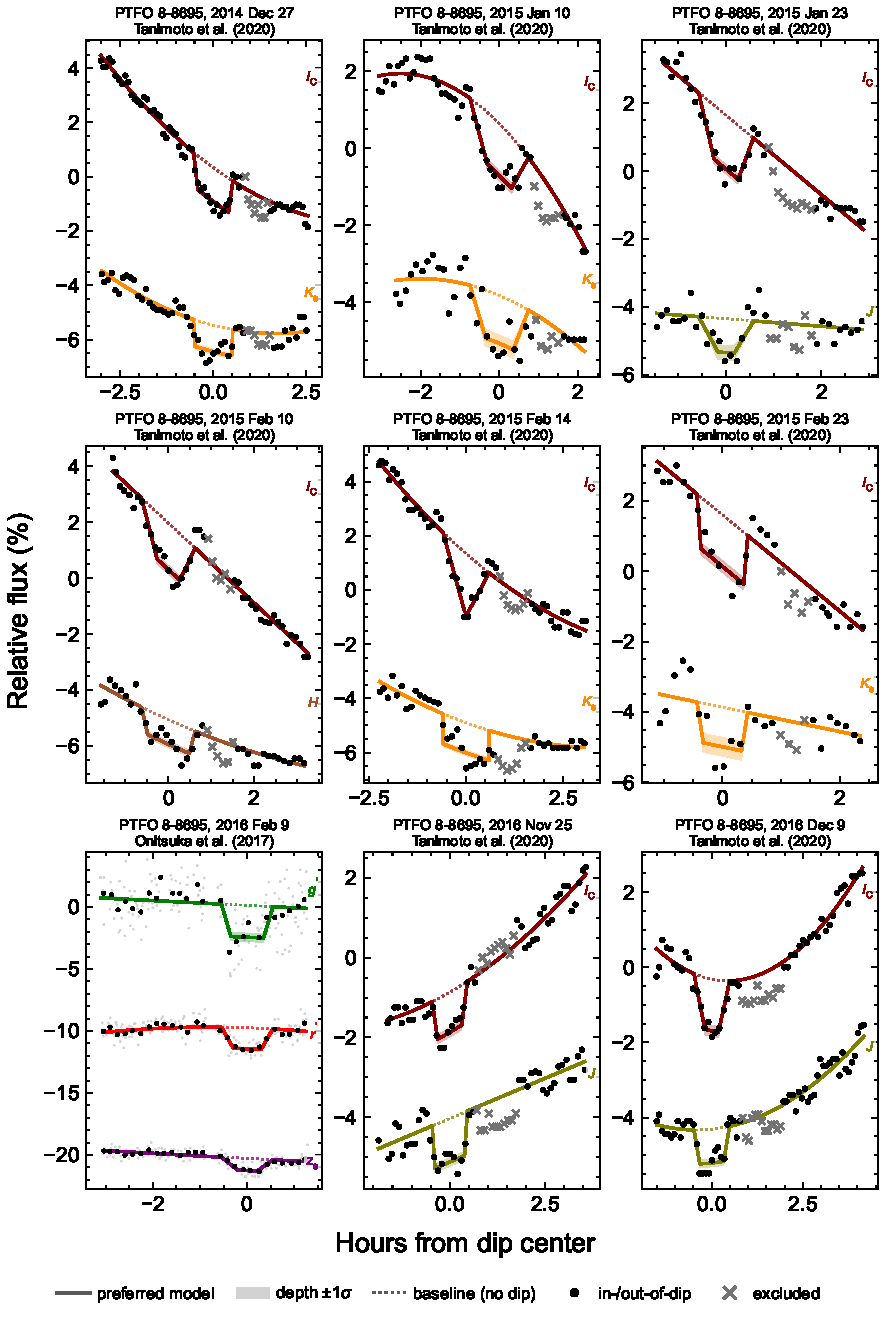
\includegraphics[width=0.8\textwidth]{dip_fit_mosaic_2.pdf}
  \vspace{-0.2cm}
  \caption{{\bf Trapezoidal fits to multi-band photometry of CPVs
  (part 2/2).} We digitally transcribed these PTFO\,8-8695
  measurements from
  \citet{Onitsuka2017} and \citet{Tanimoto2020}.  The underplotted
  contours show our fitted $\pm$1-$\sigma$ dip depth uncertainties. }
  \label{fig:dipfit2}
\end{figure*}


%%%%%%%%%%%%%%%%%%%%%%%%%%%%%%%%%%%%%%%%%%
%%%%%%%%%%%%%%%%%%%%%%%%%%%%%%%%%%%%%%%%%%

%\clearpage

\bibliographystyle{aasjournalv7}
\bibliography{cpvbib.bib}

%%%%%%%%%%%%%%%%%%%%%%%%%%%%%%%%%%%%%%%%%%
%%%%%%%%%%%%%%%%%%%%%%%%%%%%%%%%%%%%%%%%%%

\end{document}



